% $Id: faq-how-do-i.tex,v 1.47 2014/01/28 18:17:23 rf10 Exp $

\section{How do I do\dots{}?}

\subsection{Mathematics}

\Question[Q-proof]{Proof environment}

It was long thought impossible to make a \environment{proof}
environment which automatically includes an `end-of-proof' symbol.
Some proofs end in displayed maths; others do not.  If the input file
contains % ! line break
\texttt{...\csx{]} }\cmdinvoke{end}{proof} then \LaTeX{} finishes off
the displayed maths and gets ready for a new line before it reads any
instructions connected with ending the proof, so the code is very
tricky.  You \emph{can} insert the symbol by hand, but the
(apparently) original `automatic' solution came with Paul Taylor's
\Package{QED}.

Nowadays, the \Package{ntheorem} package now solves the problem for
\LaTeX{} users: it provides an automatic way of signalling
the end of a proof.

The \AMSLaTeX{} package \Package{amsthm} also provides a
\environment{proof} environment that does the job; though you need to
insert a \csx{qedhere} command if the proof ends with a displayed
equation:
\begin{quote}
\begin{verbatim}
\begin{proof}
  text...
  \begin{equation*}
    maths... \tag*{\qedhere}
  \end{equation*}
\end{proof}
\end{verbatim}
\end{quote}
The \cmdinvoke{tag*}{\csx{qedhere}} construction may be used in any of
\AMSLaTeX{}'s numbering environments.
\begin{ctanrefs}
\item[amsthm.sty]Distributed as part of the \AMSLaTeX{} bundle
  \CTANref{amslatex}[amsthm]
\item[ntheorem.sty]\CTANref{ntheorem}
\end{ctanrefs}
\LastEdit{2011-03-09}

\Question[Q-theoremfmt]{Theorem bodies printed in a roman font}

If you want to take advantage of the powerful \csx{newtheorem} command
without the constraint that the contents of the theorem is in a sloped
font (for example, you may want to use it to create remarks, examples, proofs,
\dots{}) then you can use the \AMSLaTeX{} \Package{amsthm} package
(which now supersedes the \Package{theorem} package previously
recommended in these answers).
Alternatively, the following sets up an environment
\environment{remark} whose content is in the default roman font.
\begin{quote}
\begin{narrowversion}
\begin{verbatim}
\newtheorem{preremark}{Remark}
\newenvironment{remark}%
  {\begin{preremark}\upshape}%
  {\end{preremark}}
\end{verbatim}
\end{narrowversion}
\begin{wideversion}
\begin{verbatim}
\newtheorem{preremark}{Remark}
\newenvironment{remark}%
  {\begin{preremark}\upshape}{\end{preremark}}
\end{verbatim}
\end{wideversion}
\end{quote}
The \Package{ntheorem} package provides control of the fonts used by
theorems, directly.
\begin{ctanrefs}
\item[amsthm.sty]Distributed as part of \CTANref{amslatex}[amsthm]
\item[ntheorem.sty]\CTANref{ntheorem}
\item[theorem.sty]Distributed as part of \CTANref{2etools}[theorem]
\end{ctanrefs}

\Question[Q-newfunction]{Defining a new log-like function in \LaTeX{}}

Use the \csx{mathop} command, as in:
\begin{quote}
\begin{verbatim}
\newcommand{\diag}{\mathop{\mathrm{diag}}}
\end{verbatim}
\end{quote}

Subscripts and superscripts on \csx{diag} will be placed below and
above the function name, as they are on
\csx{lim}.  If you want your subscripts and superscripts always placed
to the right, do:
\begin{quote}
\begin{narrowversion}
\begin{verbatim}
\newcommand{\diag}%
  {\mathop{\mathrm{diag}}\nolimits}
\end{verbatim}
\end{narrowversion}
\begin{wideversion}
\begin{verbatim}
\newcommand{\diag}{\mathop{\mathrm{diag}}\nolimits}
\end{verbatim}
\end{wideversion}
\end{quote}

\AMSLaTeX{} (in its \Package{amsopn} package, which is automatically
loaded by \Package{amsmath}) provides a command
\csx{DeclareMathOperator} that takes does the same job as the first
definition above.  To create our original \csx{diag} command, one would
say:
\begin{quote}
\begin{verbatim}
\DeclareMathOperator{\diag}{diag}
\end{verbatim}
\end{quote}
\csx{DeclareMathOperator*} declares the operator always to have its
sub- and superscripts in the % ! line break
``\Qref*{\csx{limits} position}{Q-limits}''.

The \Package{amsopn} command \csx{operatorname} allows you to
introduce \emph{ad hoc} operators into your mathematics, so
\begin{quote}
  \csx{[} \cmdinvoke{operatorname}{foo}\texttt{(bar)} \csx{]}
\end{quote}
typesets the same as
\begin{quote}
\begin{verbatim}
\DeclareMathOperator{\foo}{foo}
...
\[ \foo(bar) \]
\end{verbatim}
\end{quote}
As with \csx{DeclareMathOperator} there's a starred version
\csx{operatorname*} for sub- and superscripts in the limits position.

(It should be noted that ``log-like'' was reportedly a \emph{joke} on
Lamport's part; it is of course clear what was meant.)
\begin{ctanrefs}
\item[amsopn.sty]Distributed as part of the \AMSLaTeX{} distribution
  \CTANref{amslatex}[amsopn]
\end{ctanrefs}

\Question[Q-braket]{Set specifications and Dirac brackets}

One of the few glaring omissions from \TeX{}'s mathematical
typesetting capabilities is a means of setting separators in the
middle of mathematical expressions.  \TeX{} provides primitives called
\csx{left} and \csx{right}, which can be used to modify brackets (of
whatever sort) around a mathematical expression, as in:
% beware line wrap
\csx{left(}\texttt{ <expression> }\csx{right)}~--- the size of the
parentheses is matched to the vertical extent of the expression.

However, in all sorts of mathematical enterprises one may find oneself
needing a \csx{middle} command, to be used in expressions like
\begin{quote}
\begin{wideversion}
\begin{verbatim}
\left\{ x \in \mathbb{N} \middle| x \mbox{ even} \right\}
\end{verbatim}
\end{wideversion}
\begin{narrowversion}
\begin{verbatim}
\left\{ x\in \mathbb{N} \middle| 
                 x \mbox{ even} \right\}
\end{verbatim}
\end{narrowversion}
\end{quote}
to specify the set of even natural numbers.  The % ! line break
\Qref*{\eTeX{} system}{Q-etex}
defines just such a command, but users of Knuth's original need some
support.  Donald Arseneau's \Package{braket} package provides commands
for set specifications (as above) and for Dirac brackets (and bras and
kets).  The package uses the \eTeX{} built-in command if it finds
itself running under \eTeX{}.
\begin{ctanrefs}
\item[braket.sty]\CTANref{braket}
\end{ctanrefs}

\Question[Q-cancellation]{Cancelling terms in maths expressions}

A technique used when explaining the behaviour of expressions or
equations (often for pedagogical purposes).  The \Package{cancel}
package provides several variants of cancellation marks
(``\texttt{\textbackslash }'', ``\texttt{/}'' and ``\texttt{X}''), and
a means of cancelling `to' a particular value.

Documentation of \Package{cancel} is in the package file.
\begin{ctanrefs}
\item[cancel.sty]\CTANref{cancel}
\end{ctanrefs}

\Question[Q-mathsize]{Adjusting maths font sizes}

In \plaintex{}, when you introduce a new font size you must also
declare what size fonts are to be used in mathematics with it.  This
is done by declaring \csx{textfont}, \csx{scriptfont} and
\csx{scriptscriptfont} for the maths families you're using; all such
things are described in chapter~17 of the % line wrap!
\Qref*{\TeX{}book}{Q-tex-books} and in other books and
\Qref*{tutorials}{Q-man-tex} that discuss \plaintex{} in sufficient
detail.

In \LaTeX{}, of course, all this stuff is automated: there is a scheme
that, for each (text) font size, determines what maths font sizes are
to be used.  The scheme first checks a set of ``known'' text sizes,
for each of which maths sizes are declared in advance.  If the text
size isn't ``known'', the script- and scriptscriptfont sizes are
calculated as fixed ratios of the tex font size.  (The values used are
\csx{defaultscriptratio}\ensuremath{=}0.7, and
\csx{defaultscriptscriptratio}\ensuremath{=}0.5.)

The fixed-ratio formula is capable of producing inconvenient results
(particularly if you are using fonts which \LaTeX{} believes are only
available in a fixed set of sizes).  You may also want to replace
\LaTeX{}'s ideas altogether, for example by setting maths noticeably
larger or smaller than its surrounding text.  For this purpose, the
\LaTeX{} command
\cmdinvoke{DeclareMathSizes}{\meta{tfs}}{\meta{ts}}{\meta{ss}}{\meta{sss}}
may be used (this is the same command that \LaTeX{} itself uses to
define its own set of sizes).  This establishes (or re-establishes)
the maths font sizes to be used when the surrounding text font size is
\texttt{\meta{tfs}}; (\texttt{\meta{ts}} being the size used for
\csx{textfont}, \texttt{\meta{ss}} for \csx{scriptfont} and
\texttt{\meta{sss}} for \csx{scriptscriptfont}).

For example, you might want to use a font with a smaller body height
than Computer Modern, but still prefer \acro{CM} math to any of the
alternatives.  In this case, you might use:
\begin{quote}
\begin{verbatim}
\DeclareMathSizes{10}{9}{7}{5}
\end{verbatim}
\end{quote}
to get 9pt maths when the surrounding body text is (nominal) 10pt.

\csx{DeclareMathSizes} may only be used in the preamble of the
document: only one association is available for each text font size
for the whole document.  The default settings are specified in
\File{fontdef.dtx} in the latex distribution, and are compiled into
\File{fontmath.ltx}; the arguments to the command are just numbers
(`\texttt{pt}' is assumed), but some of them are written using
\Qref*{\LaTeX{} abbreviations}{Q-ltxabbrv} for standard font sizes.
Beware simply copying (parts of) the \LaTeX{} definitions~--- since
they contain those internal abbreviations, they need to be treated as
\Qref{internal commands}{Q-atsigns}.
\begin{ctanrefs}
\item[fontdef.dtx]\CTANref{fontdef}
\item[fontmath.ltx]\CTANref{fontmath}
\end{ctanrefs}
\LastEdit{2011-06-01}

\Question[Q-mathlips]{Ellipses}
\keywords{\csx{dots} \csx{cdots} \csx{vdots} \csx{ddots}}

Ellipses are commonly required, and \LaTeX{} natively supplies a fair
range (\csx{dots}, \csx{cdots}, \csx{vdots} and \csx{ddots}).  By using
the \Package{graphics} package, one can change the slope of the
\csx{ddots} command, as in
\begin{quote}
\begin{verbatim}
$ ... \reflectbox{$\ddots$} ... $
\end{verbatim}
\end{quote}
While this works, it is not a recommended way of achieving the desired
result (see below).  Moreover, \LaTeX{}'s range is not adequate to
everyone's requirements, and at least three packages provide
extensions to the set.

The \AMSLaTeX{} bundle provides a range of ``semantically-named''
ellipses, for use in different situations: \csx{dotsb} for use between
pairs of binary operators, \csx{dotsc} for use between pairs of commas,
and so on.

The \Package{yhmath} package defines an \csx{adots} command, which is
the analogue of \csx{ddots}, sloping forwards rather than backwards.
The \Package{yhmath} package comes with a rather interesting font that
extends the standard \Package{cmex}; details are in the documentation.

The \Package{mathdots} package (besides fixing up the behaviour of
\AllTeX{} \csx{ddots} and \csx{vdots} when the font size changes)
provides an ``inverse diagonal'' ellipsis \csx{iddots} (doing the same
job as \Package{yhmath}'s \csx{adots}, but better).

Documentation of \Package{yhmath} appears, processed, in the
distribution (thus saving you the bother of installing the package
before being able to read the documentation).  Documentation of
\Package{mathdots} appears at the end the package file itself.
\begin{ctanrefs}
\item[amslatex]\CTANref{amslatex}
\item[graphics.sty]Part of the \CTANref{graphics} bundle
\item[mathdots.sty]\CTANref{mathdots}
\item[yhmath]\CTANref{yhmath}
\end{ctanrefs}
\LastEdit{2013-08-21}

\Question[Q-limits]{Sub- and superscript positioning for operators}

The commonest hand-written style for expressions is to place the limit
expressions on operators such as \csx{sum} and \csx{int} physically
above and below the operator.  In \AllTeX{}, we write these limit
expressions using sub- and superscripts applied to the operator, but
they don't always appear in the ``handwritten'' way in \TeX{}'s
output.

The reason is, that when an expression appears in non-display maths,
in running text (and is therefore in \TeX{} \csx{textstyle}), placing
the limits thus could lead to ragged line spacing (and hence
difficult-to-read text).  It is therefore common (in \csx{textstyle})
to place the limits as one would sub- and superscripts of variables.

This is not universally satisfactory, so the primitive \csx{limits} is
provided:
\begin{quote}
\begin{verbatim}
$\sum\limits_{n=1}^{m} ...$
\end{verbatim}
\end{quote}
which will place the limits right above and below the symbol (and be
blowed to the typography\dots{}).

Contrariwise, you may wish to change the arrangement of the limits
when in \csx{displaystyle}.  For this purpose, there's a corresponding
\csx{nolimits}:
\begin{quote}
\begin{verbatim}
\[\sum\nolimits_{n=1}^{m} ...\]
\end{verbatim}
\end{quote}
which will place the limits as they would be in \csx{textstyle}.

Alternatively, one can manipulate the
\csx{textstyle}/\csx{displaystyle} state of the mathematics.  To get
``\csx{limits} placement'' in inline maths,
\begin{quote}
\begin{verbatim}
$\displaystyle\sum_{n=1}^{m} ...$
\end{verbatim}
\end{quote}
and for ``\csx{nolimits} placement'' in display maths,
\csx{nolimits}:
\begin{quote}
\begin{verbatim}
\[\textstyle\sum_{n=1}^{m} ...\]
\end{verbatim}
\end{quote}
will serve.  Either of these forms may have effects other than on the
operator you're considering, but there are still those who prefer this
formulation.

Remember, if you're % ! line break
\Qref*{declaring a special operator of your own}{Q-newfunction}, the
\AMSLaTeX{} functions (that you ought to be using) allow you to choose
how limits are displayed, at definition time.

(Note that the macro \csx{int} normally has \csx{nolimits} built in to
its definition.  There is an example in the \TeX{}book to show how odd
\csx{int}\csx{limits} looks when typeset.)

\Question[Q-mathstext]{Text inside maths}

When we type maths in \AllTeX{}, the letters from which we make up
ordinary text assume a special significance: they all become
single-letter variable names.  The letters appear in italics, but it's
not the same sort of italics that you see when you're typing ordinary
text: a run of maths letters (for example ``here'') looks oddly
``lumpy'' when compared with the word written in italic text.  The
difference is that the italic text is kerned to make the letters fit
well together, whereas the maths is set to look as if you're
multiplying \emph{h} by \emph{e} by \emph{r} by \emph{e}.  The other
way things are odd in \TeX{} maths typing is that spaces are ignored:
at best we can write single words in this oddly lumpy font.

So, if we're going to have good-looking text in amongst maths we're
writing, we have to take special precautions.  If you're using
\LaTeX{}, the following should help.

The simplest is to use \csx{mbox} or \csx{textrm}:
\begin{quote}
\begin{verbatim}
$e = mc^2 \mbox{here we go again}$
\end{verbatim}
\end{quote}
The problem is that, with either, the size of the text remains firmly
at the surrounding text size, so that
\begin{quote}
\begin{verbatim}
$z = a_{\mbox{other end}}$
\end{verbatim}
\end{quote}
can look quite painfully wrong.

The other simple technique, \csx{textrm}, is no more promising:
\begin{quote}
\begin{verbatim}
$z = a_{\textrm{other end}}$
\end{verbatim}
\end{quote}
does the same as \csx{mbox}, by default.

(The maths-mode instance of your roman font (\csx{mathrm}) gets the
size right, but since it's intended for use in maths, its spaces get
ignored~--- use \csx{mathrm} for upright roman alphabetic variable
names, but not otherwise.)

You can correct these problems with size selectors in the text, as:
\begin{quote}
\begin{verbatim}
$z = a_{\mbox{\scriptsize other end}}$
\end{verbatim}
\end{quote}
which works if your surrounding text is at default document size, but
gives you the wrong size otherwise.

The \csx{mbox} short cut is (just about) \acro{OK} for ``occasional''
use, but serious mathematics calls for a technique that
relieves the typist of the sort of thought required.  As usual, the
\AMSLaTeX{} system provides what's necessary~--- the \csx{text}
command.  (The command is actually provided by the \Package{amstext}
package, but the ``global'' \Package{amsmath} package loads it.)  Thus
anyone using \AMSLaTeX{} proper has the command available, so even
this author can write:
\begin{quote}
\begin{verbatim}
\usepackage{amsmath}
...
$z = a_{\text{other end}}$
\end{verbatim}
\end{quote}
and the text will be at the right size, and in the same font as
surrounding text.  (The \Package{amstext} package also puts
\csx{textrm} to rights~--- but \csx{text} is easier to type than
\csx{textrm}!)

\AMSLaTeX{} also makes provision for interpolated comments in the
middle of one of its multi-line display structures, through the
\csx{intertext} command.  For example:
\begin{quote}
\begin{narrowversion}
\begin{verbatim}
\begin{align}
  A_1&=N_0(\lambda;\Omega')-
    \phi(\lambda;\Omega'),\\
  A_2&=\phi(\lambda;\Omega')-
    \phi(\lambda;\Omega),\\
\intertext{and}
  A_3&=\mathcal{N}(\lambda;\omega).
\end{align}
\end{verbatim}
\end{narrowversion}
\begin{wideversion}
\begin{verbatim}
\begin{align}
  A_1&=N_0(\lambda;\Omega')-\phi(\lambda;\Omega'),\\
  A_2&=\phi(\lambda;\Omega')-\phi(\lambda;\Omega),\\
  \intertext{and} A_3&=\mathcal{N}(\lambda;\omega).
\end{align}
\end{verbatim}
\end{wideversion}
\end{quote}
places the text ``and'' on a separate line before the last line of the
display.  If the interjected text is short, or the equations
themselves are light-weight, you may find that \csx{intertext} leaves
too much space.  Slightly more modest is the \csx{shortintertext}
command from the \Package{mathtools} package:
\begin{quote}
\begin{verbatim}
\begin{align}
  a =& b
  \shortintertext{or}
  c =& b
\end{align}
\end{verbatim}
\end{quote}
To have the text on the same line as the second equation, one can use
the \environment{flalign} environment (from \Package{amsmath})
with lots of dummy equations (represented by the double \texttt{\&}
signs):
\begin{quote}
\begin{verbatim}
\begin{flalign}
            && a =& b && \\
  \text{or} && c =& b &&
\end{flalign}
\end{verbatim}
\end{quote}
\begin{ctanrefs}
\item[amsmath.sty]Distributed as part of \AMSLaTeX{}
  \CTANref{amslatex}[amsmath]
\item[amstext.sty]Distributed as part of \AMSLaTeX{}
  \CTANref{amslatex}[amstext]
\item[mathtools.sty]Distributed as part of the \Package{mh} bundle
  \CTANref{mh}[mathtools]
\end{ctanrefs}

\Question[Q-reuseq]{Re-using an equation}

To repeat an existing equation, one wants not only to have the same
mathematics in it, one also wants to re-use the original label it had.
The \Package{amsmath} package comes to our help, here:
\begin{quote}
\begin{verbatim}
\usepackage{amsmath}
...
\begin{equation}
  a=b
  \label{eq1}
\end{equation}
...
Remember that
\begin{equation}
  a=b
  \tag{\ref{eq1}}
\end{equation}
\end{verbatim}
\end{quote}
Here, the second instance of \ensuremath{a=b} will be
typeset with a copy, made by the \csx{tag} command, of the label of the
first instance.
\begin{ctanrefs}
\item[amsmath.sty]Distributed as part of \AMSLaTeX{}
  \CTANref{amslatex}[amsmath]
\end{ctanrefs}

\Question[Q-brkinline]{Line-breaking in in-line maths}

\TeX{}, by default, allows you to split a mathematical expression at
the end of the line; it allows breaks at relational operators (like
``='', ``\textless'', etc.) and at binary operators (like ``+'',
``-'', etc.).  In the case of large expressions, this can sometimes be
a life-saver.

However, in the case of simple expressions like \ensuremath{a=b+c}, a
break can be really disturbing to the reader, and one would like to
avoid it.

Fortunately, these breaks are controllable: there are ``penalties''
associated with each type of operator: the penalty 
 says how
undesirable a break at each point is.  Default values are:
\begin{quote}
\begin{verbatim}
\relpenalty   = 500
\binoppenalty = 700
\end{verbatim}
\end{quote}
You make the break progressively less attractive by increasing these
values.  You can actually forbid all breaks, everywhere, by:
\begin{quote}
\begin{verbatim}
\relpenalty   = 10000
\binoppenalty = 10000
\end{verbatim}
\end{quote}
If you want just to prevent breaks in a single expression, write:
\begin{quote}
\begin{verbatim}
{%
  \relpenalty   = 10000
  \binoppenalty = 10000
  $a=b+c$
}
\end{verbatim}
\end{quote}
and the original values will remain undisturbed outside the braces.
This is tedious: there is often value in an alternative approach,
in which you say which parts of the expression may not break whatever
happens, and fortunately this is surprisingly easy.  Suppose we want
to defer a break until after the equality, we could write:
\begin{quote}
\begin{verbatim}
${a+b+c+d} = z+y+x+w$
\end{verbatim}
\end{quote}
The braces say ``treat this subformula as one atom'' and (in \TeX{} at
least) atoms don't get split: not a \csx{binoppenalty} change in sight.

\Question[Q-mathonlyref]{Numbers for referenced equations only}

There are those who consider that papers look untidy with numbers on
every equation; there is also a school of thought that claims that
there should be numbers everywhere, in case some reader wants to make
reference an equation to which the author made no cross-reference.

If you hold to the ``only cross-referenced'' school of thought, you
can (using the \csx{nonumber} command on the relevant equations, or by
using the \AMSLaTeX{} unnumbered environments such as
\environment{equation*}) mark those of your equations to which you
make no reference.  In a long or complex paper, this procedure could
well become deeply tedious.

Fortunately, help is at hand: the \Package{mh} bundle's
\Package{mathtools} package offers a `\pkgoption{showonlyrefs}'
switch through its \csx{mathtoolsset} command; when that's in
operation, only those equations to which you make reference will be
numbered in the final output.  See the package's documentation for
details of how to make references when the switch is in effect.
\begin{ctanrefs}
\item[mathtools.sty]Distributed as part of \CTANref{mh}[mathtools]
\end{ctanrefs}

\Question[Q-subheight]{Even subscript height}

Other things being equal, \TeX{} will aim to position subscripts and
superscripts in places that ``look good''.  Unfortunately, it only
does this for the sub- and superscripts of each atom at a time, so if
you have
\begin{quote}
\begin{verbatim}
$ X^{1}_{2} X_{2} $
\end{verbatim}
\end{quote}
the second subscript will appear higher, since the first has moved
down to avoid the superscript;
the effect can be noticeably distracting:
\begin{quote}
\begin{typesetversion}
  $ X^{1}_{2} X_{2} $
\end{typesetversion}
\begin{htmlversion}
  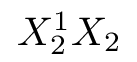
\includegraphics{faq-images1.png}
\end{htmlversion}
\end{quote}

You can avoid the problem, for a single instance, by
\begin{quote}
\begin{verbatim}
$ X^{1}_{2} X^{}_{2} $
\end{verbatim}
\end{quote}
here, the dummy superscript has the requisite ``pushing down'' effect:
\begin{quote}
\begin{typesetversion}
  $ X^{1}_{2} X^{}_{2} $
\end{typesetversion}
\begin{htmlversion}
  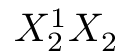
\includegraphics{faq-images2.png}
\end{htmlversion}
\end{quote}

While this technique does what is necessary, it is tedious and
potentially error-prone.  So, for more than one or two equations
in a document, the \LaTeX{} user is advised to use the
\Package{subdepth} package, which forces the lower position for all
subscripts.
\begin{ctanrefs}
\item[subdepth.sty]\CTANref{subdepth}
\end{ctanrefs}

\subsection{Lists}

\Question[Q-enumerate]{Fancy enumeration lists}

The \Package{enumerate} package allows you to control the display of
the enumeration counter.  The package adds an optional parameter to
the \environment{enumerate} environment, which is used to specify the
layout of the labels.  The layout parameter contains an enumeration
type (`\texttt{1}' for arabic numerals, `\texttt{a}' or `\texttt{A}'
for alphabetic enumeration, and `\texttt{i}' or `\texttt{I}' for Roman
numerals), and things to act as decoration of the enumeration.  So,
for example
\begin{quote}
\begin{verbatim}
\usepackage{enumerate}
...
\begin{enumerate}[(a)]
\item ...  ...
\end{enumerate}
\end{verbatim}
\end{quote}
starts a list whose labels run (a), (b), (c), \dots{}; while
\begin{quote}
\begin{verbatim}
\usepackage{enumerate}
...
\begin{enumerate}[I/]
\item ...  ...
\end{enumerate}
\end{verbatim}
\end{quote}
starts a list whose labels run I/, II/, III/, \dots{}

The \Package{paralist} package, whose primary purpose is % beware line break
\Qref*{compaction of lists}{Q-complist}, provides the same facilities
for its \environment{enumerate}-like environments.

If you need non-stereotyped designs, the \Package{enumitem} package
gives you most of the flexibility you might want to design your own.
The silly roman example above could be achieved by:
\begin{quote}
\begin{verbatim}
\usepackage{enumitem}
...
\begin{enumerate}[label=\Roman{*}/]
\item ...  ...
\end{enumerate}
\end{verbatim}
\end{quote}
Note that the `\texttt{*}' in the key value stands for the list
counter at this level.  You can also manipulate the format of
references to list item labels:
\begin{quote}
\begin{narrowversion}
\begin{verbatim}
\usepackage{enumitem}
...
\begin{enumerate}[label=\Roman{*}/,
  ref=(\roman{*})]
\item ...  ...
\end{enumerate}
\end{verbatim}
\end{narrowversion}
\begin{wideversion}
\begin{verbatim}
\usepackage{enumitem}
...
\begin{enumerate}[label=\Roman{*}/, ref=(\roman{*})]
\item ...  ...
\end{enumerate}
\end{verbatim}
\end{wideversion}
\end{quote}
to make references to the list items format appear as (i), (ii),
(iii), etc.

The \Class{memoir} class includes functions that match those in the
\Package{enumerate} package, and has similar functionality for
\environment{itemize} lists.
%% It is possible (if not particularly convenient) to do the same thing
%% yourself.  Suppose you want your top-level \environment{enumerate}s to
%% be labelled I/, II/, III/, \dots{}, then give these commands:
%% \begin{verbatim}
%%    \renewcommand{\theenumi}{\Roman{enumi}}
%%    \renewcommand{\labelenumi}{\theenumi/}
%% \end{verbatim}
%% The possible styles of numbering are given in Section~6.3 of Lamport's
%% book (see \Qref[question]{\TeX{}-related books}{Q-book-lists}).  Both
%% \csx{theenumi} and \csx{labelenumi} must be changed, since
%% \csx{theenumi} is used in cross-references to the list.
%%
%% For lower level \environment{enumerate}s, replace |enumi| by |enumii|,
%% |enumiii| or |enumiv|, according to the level.  If your label is much
%% larger than the default, you should also change \csx{leftmargini},
%% \csx{leftmarginii}, \emph{etc}.
\begin{ctanrefs}
\item[enumerate.sty]Distributed as part of \CTANref{2etools}[enumerate]
\item[enumitem.sty]\CTANref{enumitem}
\item[memoir.cls]\CTANref{memoir}
\item[paralist.sty]\CTANref{paralist}
\end{ctanrefs}

\Question[Q-complist]{How to adjust list spacing}

\Qref*{Lamport's book}{Q-latex-books} lists various
parameters for the layout of list (things like \csx{topsep},
\csx{itemsep} and \csx{parsep}), but fails to mention that they're set
automatically within the standard (\LaTeX{}-defined) lists.  This
happens because each list
executes a command \csx{@list}\texttt{\meta{depth}} (the depth
appearing as a lower-case roman numeral); what's more, the top-level
\csx{@listi} is usually reset when the font size is changed.  As a
result, it's rather tricky for 
the user to control list spacing.  Of course, the real answer is to use
a document class designed with more modest list spacing, but we all
know such things are hard to come by.  The \Class{memoir} class doesn't
provide more compact lists, but offers the user control over the list
spacing using \csx{firmlist} and \csx{tightlist} (and \texttt{*}-ed
versions of them); see section~8.6 of the memoir manual.

There are packages that provide some control of list spacing, but they
seldom address the separation from surrounding text (defined by
\csx{topsep}).  The \Package{expdlist} package, among its many controls
of the appearance of \environment{description} lists, offers a
compaction parameter (see the documentation); the \Package{mdwlist}
package offers a \csx{makecompactlist} command for users' own list
definitions, and uses it to define compact lists
\environment{itemize*}, \environment{enumerate*} and
\environment{description*}.  In fact, you can write lists such as
these commands define pretty straightforwardly~--- for example:
\begin{quote}
\begin{verbatim}
\newenvironment{itemize*}%
  {\begin{itemize}%
    \setlength{\itemsep}{0pt}%
    \setlength{\parskip}{0pt}}%
  {\end{itemize}}
\end{verbatim}
\end{quote}
The \Package{paralist} package provides several approaches to list
compaction:
\begin{itemize}
\item its \environment{asparaenum} environment formats each item as if
  it were a paragraph introduced by the enumeration label (which saves
  space if the item texts are long);
\item its \environment{compactenum} environment is the same sort of
  compact list as is provided in \Package{expdlist} and
  \Package{mdwlist}; and
\item its \environment{inparaenum} environment produces a list ``in
  the paragraph'', i.e., with no line break between items, which is a
  great space-saver if the list item texts are short.
\end{itemize}
The package will manipulate its \environment{enumerate} environment
labels just like the \Qref*{\Package{enumerate} package}{Q-enumerate}
does.

\Package{Paralist} also provides \environment{itemize} equivalents
(\environment{asparaitem}, etc.), and \environment{description}
equivalents (\environment{asparadesc}, etc.).

The \Package{multenum} package offers a more regular form of
\Package{paralist}'s \environment{inparaenum}; you define a notional
grid on which list entries are to appear, and list items will always
appear at positions on that grid.  The effect is somewhat like that of
the `tab' keys on traditional typewriters; the package was designed
for example sheets, or lists of answers in the appendices of a book.

The \Package{expdlist}, \Package{mdwlist} and \Package{paralist}
packages all offer other facilities for list configuration: you should
probably not try the ``do-it-yourself'' approaches outlined below if
you need one of the packages for some other list configuration
purpose.

For ultimate flexibility (including manipulation of \csx{topsep}), the
\Package{enumitem} package permits adjustment of list parameters using
a ``\emph{key}\latexhtml{\ensuremath{=}}{=}\meta{value}'' format.
For example, one might write
\begin{quote}
\begin{verbatim}
\usepackage{enumitem}
...
\begin{enumerate}[topsep=0pt, partopsep=0pt]
\item ...
\item ...
\end{enumerate}
\end{verbatim}
\end{quote}
to suppress all spacing above and below your list, or
\begin{quote}
\begin{verbatim}
\usepackage{enumitem}
...
\begin{enumerate}[itemsep=2pt,parsep=2pt]
\item ...
\item ...
\end{enumerate}
\end{verbatim}
\end{quote}
to set spacing between items and between paragraphs within items.
\Package{Enumitem} also permits manipulation of the label format in a
more ``basic'' (and therefore more flexible) manner than the % ! line break
\Qref*{\Package{enumerate} package}{Q-enumerate} does.

The ultimate in compaction (of every sort) is offered by the
\Package{savetrees} package; compaction of lists is included.  The
package's prime purpose is to save space at every touch and turn:
don't use it if you're under any design constraint whatever!
\begin{ctanrefs}
\item[enumerate.sty]Distributed as part of \CTANref{2etools}[enumitem]
\item[enumitem.sty]\CTANref{enumitem}
\item[expdlist.sty]\CTANref{expdlist}
\item[memoir.cls]\CTANref{memoir}
\item[memoir \nothtml{\rmfamily}manual]\CTANref{memoir-man}
\item[mdwlist.sty]Distributed as part of \CTANref{mdwtools}[mdwlist]
\item[multenum.sty]\CTANref{multenum}
\item[paralist.sty]\CTANref{paralist}
\item[savetrees.sty]\CTANref{savetrees}
\end{ctanrefs}
\LastEdit{2012-10-30}

\Question[Q-interruptlist]{Interrupting enumerated lists}

It's often convenient to have commentary text, `outside' the list,
between successive entries of a list.  In the case of
\environment{itemize} lists this is no problem, since there's never
anything to distinguish successive items, while in the case of
\environment{description} lists, the item labels are under the user's
control so there's no automatic issue of continuity.

For \environment{enumerate} lists, the labels are generated
automatically, and are context-sensitive, so the context (in this
case, the state of the enumeration counter) needs to be preserved.

The belt-and-braces approach is to remember the state of the
enumeration in your own counter variable, and then restore it when
restarting enumerate:
\begin{quote}
\begin{verbatim}
\newcounter{saveenum}
 ...
\begin{enumerate}
  ...
  \setcounter{saveenum}{\value{enumi}}
\end{enumerate}
<Commentary text>
\begin{enumerate}
  \setcounter{enumi}{\value{saveenum}}
  ...
\end{enumerate}
\end{verbatim}
\end{quote}

This is reasonable, in small doses\dots{} Problems (apart from sheer
verbosity) are getting the level right (``should I use counter
\texttt{enumi}, \texttt{enumii}, \dots{}'') and remembering not to
nest the interruptions (i.e., not to have a separate list, that is
itself interrupted) in the ``commentary text'').

The \Package{mdwlist} package defines commands \csx{suspend} and
\csx{resume} that simplify the process:
\begin{quote}
\begin{verbatim}
\begin{enumerate}
  ...
\suspend{enumerate}
<Commentary text>
\resume{enumerate}
  ...
\end{enumerate}
\end{verbatim}
\end{quote}
The package allows an optional name (as in
\cmdinvoke{suspend}[id]{enumerate}) to allow you to identify a
particular suspension, and hence provide a handle for manipulating
nested suspensions.

If you're suspending a \Qref*{fancy-enumeration list}{Q-enumerate},
you need to 
re-supply the optional ``item label layout'' parameters required by
the \Package{enumerate} package when resuming the list, whether by the
belt-and-braces approach, or by the \Package{mdwlist}
\cmdinvoke{resume}{enumerate} technique.  The task is a little tedious
in the \Package{mdwlist} case, since the optional argument has to be
encapsulated, whole, inside an optional argument to \csx{resume},
which requires use of extra braces:
\begin{quote}
\begin{verbatim}
\begin{enumerate}[\textbf{Item} i]
  ...
\suspend{enumerate}
<comment>
\resume{enumerate}[{[\textbf{Item} i]}]
...
\end{enumerate}
\end{verbatim}
\end{quote}
\nothtml{\noindent}The \Package{enumitem} package, in its most recent
release, will also allow you to resume lists:
\begin{quote}
\begin{verbatim}
\begin{enumerate}
...
\end{enumerate}
<comment>
\begin{enumerate}[resume]
...
\end{enumerate}
\end{verbatim}
\end{quote}
which feels just as ``natural'' as the \Package{mdwtools} facility,
and has the advantage of playing well with the other excellent
facilities of \Package{enumitem}.

\Package{Expdlist} has a neat way of providing for comments, with its
\csx{listpart} command.  The command's argument becomes a comment
between items of the list:
\begin{quote}
\begin{verbatim}
\begin{enumerate}
\item item 1
\item item 2
  \listpart{interpolated comment}
\item item 3
\end{enumerate}
\end{verbatim}
\end{quote}
This, you will realise, means it doesn't even have to think about
suspending or resuming the list, and of course it works equally well
in any of the list environments (thought it's not actually
\emph{necessary} for any but \environment{enumerate}).

\Package{Enumitem} also allows multi-level suspension and resumption
of lists:
\begin{quote}
\begin{verbatim}
\begin{enumerate}
\item outer item 1
\end{enumerate}
<comment>
\begin{enumerate}[resume]
\item outer item 2
% nested enumerate
\begin{enumerate}
\item inner item 1
\end{enumerate}
<nested comment>
% resume nested enumerate
\begin{enumerate}[resume]
\item inner item 2
\end{enumerate}
\item outer item 3
% end outer enumerate
\end{enumerate}
\end{verbatim}
\end{quote}
However, the `nested comment' interpolated in the nested enumeration
appears as if it were a second paragraph to ``outer item 2'', which is
hardly satisfactory.
\begin{ctanrefs}
\item[enumerate.sty]Distributed as part of \CTANref{2etools}[enumerate]
\item[enumitem.sty]\CTANref{enumitem}
\item[expdlist.sty]\CTANref{expdlist}
\item[mdwlist.sty]Distributed as part of \CTANref{mdwtools}[mdwlist]
\end{ctanrefs}

\subsection{Tables, figures and diagrams}

\Question[Q-destable]{The design of tables}

In recent years, several authors have argued that the examples, set
out by Lamport in his \Qref*{\LaTeX{} manual}{Q-latex-books}, have cramped
authors' style and have led to extremely poor table design.  It is in
fact difficult even to work out what many of the examples in Lamport's
book ``mean''.

The criticism focuses on the excessive use of rules (both horizontal
and vertical) and on the poor vertical spacing that Lamport's macros
offer.

The problem of vertical spacing is plain for all to see, and is
addressed in several packages~--- see % beware line breaks
``\Qref*[question]{spacing of lines in tables}{Q-struttab}''.

The argument about rules is presented in the excellent essay that
prefaces the documentation of Simon Fear's \Package{booktabs} package,
which (of course) implements Fear's scheme for `comfortable' rules.
(The same rule commands are implemented in the \Class{memoir} class.)

Lamport's \LaTeX{} was also inflexibly wrong in ``insisting'' that
captions should come at the bottom of a table.  Since a table may
extend over several pages, traditional typography places the caption
at the top of a table float.  The \csx{caption} command will get its
position wrong (by \texttt{10pt}) if you simply write:
\begin{quote}
\begin{verbatim}
\begin{table}
  \caption{Example table}
  \begin{tabular}{...}
    ...
  \end{tabular}
\end{table}
\end{verbatim}
\end{quote}
The \Package{topcapt} package solves this problem:
\begin{quote}
\begin{verbatim}
\usepackage{topcapt}
...
\begin{table}
  \topcaption{Example table}
  \begin{tabular}{...}
    ...
  \end{tabular}
\end{table}
\end{verbatim}
\end{quote}
The \Class{KOMA-script} classes provide a similar command
\csx{captionabove}; they also have a class option
\pkgoption{tablecaptionabove} which arranges that \csx{caption}
\emph{means} \csx{captionabove}, in table environments.  The
\Package{caption} package may be loaded
with an option that has the same effect:
\begin{quote}
\begin{verbatim}
\usepackage[tableposition=top]{caption}
\end{verbatim}
\end{quote}
or the effect may be established after the package has been  loaded:
\begin{quote}
\begin{verbatim}
\usepackage{caption}
\captionsetup[table]{position=above}
\end{verbatim}
\end{quote}
(Note that the two ``position'' options are different: actually,
``above'' and ``top'' in these contexts mean the same thing.)

Doing the job yourself is pretty easy: \Package{topcapt} switches the
values of the \LaTeXe{} parameters \csx{abovecaptionskip} (default
value \texttt{10pt}) and \csx{belowcaptionskip} (default value
\texttt{0pt}), so:
\begin{quote}
\begin{verbatim}
\begin{table}
  \setlength{\abovecaptionskip}{0pt}
  \setlength{\belowcaptionskip}{10pt}
  \caption{Example table}
  \begin{tabular}{...}
    ...
  \end{tabular}
\end{table}
\end{verbatim}
\end{quote}
does the job (if the length values are right; the package and classes
are more careful!).
\begin{ctanrefs}
\item[booktabs.sty]\CTANref{booktabs}
\item[caption.sty]\CTANref{caption}
\item[\nothtml{\rmfamily}KOMA script bundle]\CTANref{koma-script}
\item[memoir.cls]\CTANref{memoir}
\item[topcapt.sty]\CTANref{topcapt}
\end{ctanrefs}
\LastEdit{2011-08-19}

\Question[Q-fixwidtab]{Fixed-width tables}

There are two basic techniques for making fixed-width tables in
\LaTeX{}: you can make the gaps between the columns stretch, or you
can stretch particular cells in the table.

Basic \LaTeX{} can make the gaps stretch: the \environment{tabular*}
environment takes an extra argument (before the \texttt{clpr} layout one)
which takes a length specification: you can say things like ``\texttt{15cm}''
or ``\csx{columnwidth}'' here.  You must also have an \csx{extracolsep}
command in the \texttt{clpr} layout argument, inside an \texttt{@\{\}}
directive.  So, for example, one might have
\begin{quote}
\begin{wideversion}
\begin{verbatim}
\begin{tabular*}{\columnwidth}{@{\extracolsep{\fill}}lllr}
\end{verbatim}
\end{wideversion}
\begin{narrowversion}
\begin{verbatim}
\begin{tabular*}{\columnwidth}%
  {@{\extracolsep{\fill}}lllr}
\end{verbatim}
\end{narrowversion}
\end{quote}
The \csx{extracolsep} applies to all inter-column gaps to its right as
well; if you don't want all gaps stretched, add
\cmdinvoke{extracolsep}{0pt} to cancel the original.

The \Package{tabularx} package defines an extra \texttt{clpr} column
specification, \texttt{X}; \texttt{X} columns behave as \texttt{p}
columns which expand to fill the space available.  If there's more
than one \texttt{X} column in a table, the spare space is distributed
between them.

The \Package{tabulary} package (by the same author) provides a way of
``balancing'' the space taken by the columns of a table.  The package
defines column specifications \texttt{C}, \texttt{L}, \texttt{R} and
\texttt{J}, giving, respectively, centred, left, right and
fully-justified versions of space-sharing columns.  The package
examines how long each column would be ``naturally'' (i.e., on a piece of paper of unlimited width), and
allocates space to each column accordingly.  There are ``sanity
checks'' so that really large entries don't cause everything else to
collapse into nothingness (there's a ``maximum width'' that any column
can exert), and so that tiny entries can't get smaller than a
specified minimum.  Of course, all this work means that the package
has to typeset each row several times, so things that leave
``side-effects'' (for example, a counter used to produce a row-number
somewhere) are inevitably unreliable, and should not even be tried.

The \Package{ltxtable} package combines the features of the
\Package{longtable} and \Package{tabularx} packages.  It's important
to read the documentation, since usage is distinctly odd; the
distribution contains no more than a file \File{ltxtable.tex}, which you
should process using \LaTeX{}.  Processing will give you a \File{.sty}
file as well as the \File{.dvi} or \File{.pdf} output containing the
documentation.
\begin{ctanrefs}
\item[ltxtable.sty]Distributed as part of \CTANref{carlisle}[ltxtable]
\item[tabularx.sty]Distributed as part of \CTANref{2etools}[tabularx]
\item[tabulary.sty]\CTANref{tabulary}
\end{ctanrefs}

\Question[Q-varwidcol]{Variable-width columns in tables}

This is a slightly different take on the problem addressed in
``\Qref*[question]{fixed-width tables}{Q-fixwidtab}''~--- here we have
a column whose size we can't absolutely predict when we design the
document.

While the basic techniques (the \Package{tabularx}, \Package{tabulary}
and \Package{ltxtable} packages) are the same for this problem as for the
fixed-width \emph{table} problem, there's one extra tool that we can
call to our aid, which may be preferable in some situations.

Suppose we have data in one column which we read from an external
source, and the source itself isn't entirely predictable.  The data in
the column may end up pretty narrow in every row of the table, or it
may be wide enough that the table would run over the edge of the page;
however, we don't want to make the column as wide as possible ``just
in case'', by defining a fixed size for the table.  We would like the
column to be as small as possible, but have the possibility to spread
to a maximum width and (if even that width is exceeded) turn into a
\texttt{p}-style column.

The \Package{varwidth} package, discussed in % ! line break
``\Qref*[question]{automatic sizing of minipages}{Q-varwidth}'', provides
a solution.  If you load it together with the \LaTeX{} ``required''
\Package{array} package, i.e.:
\begin{quote}
\begin{verbatim}
\usepackage{array}
\usepackage{varwidth}
\end{verbatim}
\end{quote}
\Package{varwidth} defines a new column-type ``\texttt{V}'', which you
can use as follows:
\begin{quote}
\begin{verbatim}
\begin{tabular}{l V{3.5cm} r}
  foo & blah      & bar \\
  foo & blah blah & bar \\
\end{tabular}
\end{verbatim}
\end{quote}
when the second column ends up less than 3.5cm wide;
or you can use it as follows:
\begin{quote}
\begin{verbatim}
\begin{tabular}{l V{3.5cm} r}
  foo & blah      & bar \\
  foo & blah blah & bar \\
  foo & blah blah blah blah blah blah
                  & bar \\
\end{tabular}
\end{verbatim}
\end{quote}
where the second column will end up noticeably wider, and will wrap to
a second line in the third row.
\begin{ctanrefs}
\item[array.sty]Distributed as part of \CTANref{2etools}[array]
\item[varwidth.sty]\CTANref{varwidth}
\end{ctanrefs}

\Question[Q-struttab]{Spacing lines in tables}

\AllTeX{} mechanisms for maintaining the space between lines (the
``\emph{leading}'') rely on \TeX{}'s paragraph builder, which compares
the shape of consecutive lines and adjusts the space between them.

These mechanisms can't work in exactly the same way when \AllTeX{} is
building a table, because the paragraph builder doesn't get to see the
lines themselves.  As a result, tables sometimes typeset with lines
uncomfortably close together (or occasionally ridiculously far apart).

Traditional (moving metal type) typographers would adjust the spacing
between lines of a table by use of a ``\emph{strut}'' (a metal
spacer).  A \TeX{} user can do exactly the same thing: most macro
packages define a \csx{strut} command, that defines a space appropriate
to the current size of the text; placing a \csx{strut} command at the
end of a troublesome row is the simplest solution to the problem~---
if it works.  Other solutions below are \LaTeX{}-specific, but some
may be simply translated to \plaintex{} commands.

If your table exhibits a systematic problem (i.e., every row is wrong
by the same amount) use \csx{extrarowheight}, which is defined by the
\Package{array} package:
\begin{quote}
\begin{verbatim}
\usepackage{array}% in the preamble
...
\setlength{\extrarowheight}{length}
\begin{tabular}{....}
\end{verbatim}
\end{quote}

To correct a single row whose maladjustment isn't corrected by a
\csx{strut} command, you can define your own, using
\cmdinvoke{rule}{0pt}{length}~--- which is a near approximation to the
command that goes inside a \csx{strut}.  The \Package{bigstrut} package
defines a strut command that you can use for this purpose:
\csx{bigstrut} on its own opens up both above and below the current
line; \cmdinvoke{bigstrut}[t] opens up above the line,
\cmdinvoke{bigstrut}[b] opens up below the line.

General solutions are available, however.  The \Package{tabls} package
automatically generates an appropriately-sized strut at the end of
each row.  Its disadvantages are that it's really rather slow in
operation (since it gets in the way of everything within tables) and
its (lack of) compatibility with other packages.

The \Package{makecell} package provides a command \csx{gape} that may
be used to apply strut expansion for a single cell of a table:
\begin{quote}
\begin{verbatim}
\begin{tabular}{lll}
  ... & \gape{cell contents} & ... \\
  ...
\end{tabular}
\end{verbatim}
\end{quote}
The package's similar \csx{Gape} command provides the same function,
but with optional arguments that allow you to adjust the top and
bottom adjustment.

To adjust every cell in whole tables, the
\cmdinvoke{setcellgapes}{\meta{value}} sets the adjustment value (an
optional argument of ``\texttt{t}'' or ``\texttt{b}'' restricts
adjustment to the top or bottom of each cell, respectively).  Having
issued \csx{setcellgapes}, the command \csx{makegapedcells} switches
cell expansion on, and \csx{nomakegapedcells} switches it off again.

The \Package{cellspace} package does a (possibly inferior) job by
defining a new table/array column type ``S'', which you apply to each
column specification.  So, for example,
\begin{quote}
\cmdinvoke{begin}{tabular}{l l l p{3cm}}
\end{quote}
would become
\begin{quote}
\cmdinvoke{begin}{tabular}{Sl Sl Sl Sp{3cm}}
\end{quote}
and so on.  This technique shows
promise of not interfering so much with other packages, but this
author has heard of no reports from the field.

The \Package{booktabs} package comes with a thought-provoking essay
about how tables should be designed.  Since table row-spacing problems
most often appear in collisions with rules, the author's thesis,
that \LaTeX{} users tend too often to rule their tables, is
interesting.  The package provides rule commands to support the
author's scheme, but deals with inter-row spacing too.  The most
recent release of \Package{booktabs} sports compatibility with
packages such as \Package{longtable}.
\begin{ctanrefs}
\item[array.sty]Distributed as part of \CTANref{2etools}[array]
\item[bigstrut.sty]\CTANref{bigstrut}
\item[booktabs.sty]\CTANref{booktabs}
\item[cellspace.sty]\CTANref{cellspace}
\item[makecell.sty]\CTANref{makecell}
\item[tabls.sty]\CTANref{tabls}
\end{ctanrefs}
\LastEdit{2011-05-02}

\Question[Q-longtab]{Tables longer than a single page}

Tables are, by default, set entirely in boxes of their own: as a
result, they won't split over a page boundary.  Sadly, the world keeps
turning up tables longer than a single page that we need to typeset.

For simple tables (whose shape is highly regular), the simplest
solution may well be to use the \environment{tabbing} environment,
which is slightly tedious to set up, but which doesn't force the whole alignment
onto a single page.

The \Package{longtable} package builds the whole table (in chunks), in
a first pass, and then uses information it has written to the \extension{aux}
file during later passes to get the setting ``right'' (the package
ordinarily manages to set tables in just two passes).  Since the
package has overview of the whole table at the time it's doing
``final'' setting, the table is set ``uniformly'' over its entire
length, with columns matching on consecutive pages.
\Package{longtable} has a reputation for failing to interwork with
other packages, but it does work with \Package{colortbl}, and its
author has provided the \Package{ltxtable} package to provide (most
of) the facilities of \Package{tabularx} (see
% beware line wrap
\Qref[question]{fixed-width tables}{Q-fixwidtab}) for long tables:
beware of its rather curious usage constraints~--- each long table
should be in a file of its own, and included by
\cmdinvoke*{LTXtable}{width}{file}.  Since \Package{longtable}'s
multiple-page tables can't possibly live inside floats, the package
provides for captions within the \environment{longtable} environment
itself.

A seeming alternative to \Package{ltxtable} is \Package{ltablex}; but
it is outdated and not fully functional.  Its worst problem is its
strictly limited memory capacity (\Package{longtable} is not so
limited, at the cost of much complication in its code);
\Package{ltablex} can only deal with relatively small tables, it doesn't seem
likely that support is available; but its user interface is much
simpler than \Package{ltxtable}, so if its restrictions aren't a
problem for you, it may be worth a try.

The \Package{supertabular} package starts and stops a
\environment{tabular} environment for each page of the table.  As a
result, each `page worth' of the table is compiled independently, and
the widths of corresponding columns may differ on successive pages.
However, if the correspondence doesn't matter, or if your columns are
fixed-width, \Package{supertabular} has the great advantage of doing
its job in a single run.

Both \Package{longtable} and \Package{supertabular} allow definition
of head- and footlines for the table; \Package{longtable} allows
distinction of the first and last head and foot.

The \Package{xtab} package fixes some infelicities of
\Package{supertabular}, and also provides a ``last head'' facility
(though this, of course, destroys \Package{supertabular}'s advantage
of operating in a single run).

The \Package{stabular} package provides a simple-to-use ``extension to
\environment{tabular}'' that allows it to typeset tables that run over
the end of a page; it also has usability extensions, but doesn't have
the head- and footline capabilities of the major packages.

Documentation of \Package{ltablex} is to be found in the package file.
\begin{ctanrefs}
\item[longtable.sty]Distributed as part of \CTANref{2etools}[longtable]
\item[ltablex.sty]\CTANref{ltablex}
\item[ltxtable.sty]Generate by running \CTANref{ltxtable}
\item[stabular.sty]Distributed as part of \CTANref{sttools}[stabular]
\item[supertabular.sty]\CTANref{supertabular}
\item[xtab.sty]\CTANref{xtab}
\end{ctanrefs}

\Question[Q-tabcellalign]{How to alter the alignment of tabular cells}

One often needs to alter the alignment of a tabular \texttt{p} (`paragraph')
cell, but problems at the end of a table row are common.  With a
\texttt{p} cell that looks like:
\begin{quote}
\begin{verbatim}
... & \centering blah ... \\
\end{verbatim}
\end{quote}
one is liable to encounter errors that complain about a ``misplaced
\csx{noalign}'' or ``\Qref*{extra alignment tab}{Q-altabcr}'', or the like.
The problem is that the command \texttt{\bsbs } means different things in
different circumstances: the \environment{tabular} environment
switches the meaning to a value for use in the table, and
\csx{centering}, \csx{raggedright} and \csx{raggedleft} all change the
meaning to something incompatible.  Note that the problem only
arises in the last cell of a row: since each cell is set into a box,
its settings are lost at the \texttt{\&} (or \texttt{\bsbs }) that
terminates it. 

In the old days, the actual value of \texttt{\bsbs } that the
\environment{tabular} environment uses was only available as an
internal command.  Nowadays, the value is a public command, and you
can in principle use it explicitly:
\begin{quote}
\begin{verbatim}
... & \centering blah ... \tabularnewline
\end{verbatim}
\end{quote}
(but that's a rather verbose way of doing things).

The \Package{array} package provides a command \csx{arraybackslash}
which restores \texttt{\bsbs } to its correct (within table) meaning;
the command may be used in \Package{array}'s ``field format'' preamble
specifications:
\begin{quote}
\begin{narrowversion}
\begin{verbatim}
\begin{tabular}{...%
        >{\centering\arraybackslash}%
                             p{50mm}}
...
\end{verbatim}
\end{narrowversion}
\begin{wideversion}
\begin{verbatim}
\begin{tabular}{... >{\centering\arraybackslash}p{50mm}}
...
\end{verbatim}
\end{wideversion}
\end{quote}

The \csx{tabularnewline} and \csx{arraybackslash} commands are
(somewhat) modern additions to \LaTeX{} and the \Package{array}
package, respectively.  In the unlikely event that neither is
available, the user may try the (old) solution which preserves the
meaning of \texttt{\bsbs }:
\begin{quote}
\begin{verbatim}
\newcommand\PBS[1]{\let\temp=\\%
  #1%
  \let\\=\temp
}
\end{verbatim}
\end{quote}
which one uses within a table as:
\begin{quote}
\begin{verbatim}
... & \PBS\centering blah ... \\
\end{verbatim}
\end{quote}
or in the preamble as:
\begin{quote}
\begin{verbatim}
\begin{tabular}{...>{\PBS\centering}p{5cm}}
\end{verbatim}
\end{quote}
\begin{ctanrefs}
\item[array.sty]Distributed as part of \CTANref{2etools}[array]
\end{ctanrefs}
\nothtml{\vskip 0pt plus 4ex}

\Question[Q-rulethk]{The thickness of rules in \LaTeX{} tables}

The rules in a \LaTeX{} table are by default \texttt{0.4pt} thick;
this is in fact a default built in at the lowest level, and applies to
all rules (including those separating blocks of running text).

Sometimes, however, we look at a table and find we want the rules to
stand out~--- perhaps to separate the text from the rest of the body
text, or to make the sections of the table stand out from one another.
However, a quick review of any \LaTeX{} manual will reveal no
technique for making any one rule stand out, and a little
experimentation shows that it is indeed pretty difficult to prevent
a change ``bleeding'' out to affect other rules in the same table.

If you look at what we have to say on the % ! line break
\Qref*{design of tables}{Q-destable}, elsewhere
among these \acro{FAQ}s, and you may sense that the design of \LaTeX{}
simply skipped the issues surrounding table design: \emph{that's}
presumably why there's no facilities to help you.

Specifically, the length \csx{arrayrulewidth} affects the thickness of
the rules (both horizontal and vertical) within both
\environment{tabular} and \environment{array} environments.  If you
change from the default (see above) only as far as
\begin{quote}
\begin{verbatim}
\setlength{\arrayrulewidth}{1pt}
\end{verbatim}
\end{quote}
the change is remarkably striking.  However, really quite subtle user
level programming proves incapable of changing just \emph{one} rule:
it's necessary to delve into the (rather tricky) code of \csx{hline}
and \csx{cline} themselves.

Fortunately, this job has already been done for the community: the
\Package{booktabs} package defines three different classes of rule
(\csx{toprule}, \csx{midrule} and \csx{bottomrule}), and the package
documentation offers hints on how to use them.  You are
\emph{strongly} advised to read the documentation pretty carefully.

The \Class{memoir} class includes the \Package{booktabs} package, and
repeats the documentation in its compendious manual.

Note that none of the above mentions the issue of the weight of
vertical rules (except in passing).  For the reasons, see the
documentation of the \Package{booktabs} package (again); vertical
rules in tables are in any case even more trickily coded than are
horizontal rules, and if their lack of configurability makes them
still less attractive, so much the better for the design of your
document.
\begin{ctanrefs}
\item[booktabs.sty]\CTANref{booktabs}
\item[memoir.cls]\CTANref{memoir}
\end{ctanrefs}

\Question[Q-textflow]{Flowing text around figures}

There are several \LaTeX{} packages that purport to do this, but they
all have their limitations because the \TeX{} machine isn't really
designed to solve this sort of problem.  Piet van Oostrum has
conducted a survey of the available packages; he recommends:
\begin{description}
\item[\texttt{floatflt}] \Package{floatflt} is an improved version
  (for \LaTeXe{}) of \File{floatfig.sty}, and its syntax is:
\begin{wideversion}
\begin{quote}
\begin{verbatim}
\begin{floatingfigure}[options]{width of figure}
  figure contents
\end{floatingfigure}
\end{verbatim}
\end{quote}
\end{wideversion}
\begin{narrowversion}
  \begin{quote}
    \cmdinvoke{begin}{floatingfigure}[\emph{options}]{\emph{figure width}}\\
    \mbox{}\qquad\emph{figure contents}\\
    \cmdinvoke{end}{floatingfigure}
  \end{quote}
\end{narrowversion}
There is a (more or less similar) \environment{floatingtable}
environment.

The tables or figures can be set left or right, or alternating on
even/odd pages in a double-sided document.

The package works with the \texttt{multicol} package, but doesn't work well
in the neighbourhood of list environments (unless you change your
\LaTeX{} document).
\item[\texttt{wrapfig}] \Package{wrapfig} has syntax:
\begin{wideversion}
\begin{quote}
\begin{verbatim}
\begin{wrapfigure}[height of figure in lines]{l,r,...}[overhang]{width}
  figure, caption, etc.
\end{wrapfigure}
\end{verbatim}
\end{quote}
\end{wideversion}
\begin{narrowversion}
  \begin{quote}
  \cmdinvoke{begin}{wrapfigure}\texttt{\%}\\
  \mbox{}%
  \qquad\qquad\texttt{[\emph{figure height in lines}]\%}\\
  \mbox{}%
  \qquad\qquad\texttt{\{l,r,\emph{etc}\}[\emph{overhang}]\{\emph{width}\}}\\
  \mbox{}\qquad\emph{figure, caption, etc.}\\
  \cmdinvoke{end}{wrapfigure}
  \end{quote}
\end{narrowversion}    
    The syntax of the \environment{wraptable} environment is similar.
    
    The \emph{\texttt{height}} may be omitted, in which case it will
    be calculated from the size of the figure; the package will use
    the greater of the specified and the
    actual width.  The \texttt{\{l,r,\emph{etc}.\}} parameter may
    also be specified as \texttt{i}\emph{(nside)} or
    \texttt{o}\emph{(utside)} for two-sided documents, and uppercase
    may be used to indicate that the picture should float.  The
    overhang allows the figure to be
    moved into the margin.  The figure or table will entered into the
    list of figures or tables if you use the \csx{caption} command.
    
    The environments do not work within list environments that end
    before the figure or table has finished, but can be used in a
    parbox or minipage, and in twocolumn format.
  \item[\texttt{picins}] \Package{Picins} is part of a large bundle
    that allows inclusion of pictures (e.g., with shadow boxes,
    various \MSDOS{} formats, etc.).  The command for inserting a
    picture at the start of a paragraph is:
\begin{wideversion}
  \begin{quote}
    \csx{parpic}\texttt{(width,height)(x-off,y-off)[Options][Position]\{Picture\}}\\
    \emph{Paragraph text}
  \end{quote}
\end{wideversion}
\begin{narrowversion}
  \begin{quote}
    \cmdinvoke*{picins}(width,height)(x-off,y-off)\texttt{\%}\\
    \mbox{\qquad\qquad}\texttt{[\emph{options}][\emph{position}]\%}\\
    \mbox{\qquad\qquad}\texttt{\{\emph{Picture}\}}\\
    \emph{Paragraph text}
  \end{quote}
\end{narrowversion}  
  All parameters except the \emph{Picture} are optional.  The picture
  can be positioned left or right, boxed with a rectangle, oval,
  shadowbox, dashed box, and a caption can be given which will be
  included in the list of figures.

  Unfortunately (for those of us whose understanding of German is not
  good), the documentation is in German.  Piet van Oostrum has written
  a summary in English.
\end{description}
All of the above deal insertions at one or other margin; they are able
to take advantage of the \TeX{} \csx{parshape} primitive that allows
you to adjust the margins of the text of a paragraph, by line (Knuth
provides an example of such use, with text typeset in a circle,
half-overlapping the margin, in chapter~14 of the \TeX{}book).  To
place insertions in the middle of a paragraph requires effort of an
entirely different sort; the \Package{cutwin} package does this for
you.  It requires a set of ``part line widths'' (two per line), and
typesets the ``cutout'' section of the paragraph line by line.  The
examples in the package documentation look enticing.

\plaintex{} users only have one option: \Package{figflow} (which
doesn't work in \LaTeX{}).  \Package{Figflow} only offers flowed
figures at the start of the paragraph, but it seems perfectly
functional. Syntax is
\begin{quote}
  \cmdinvoke*{figflow}{\meta{width}}{\meta{height}}{\meta{figure}}
\end{quote}
(the user is responsible for having the dimensions correct, and for
ensuring the figure fits on the page).
\begin{ctanrefs}
\item[cutwin.sty]\CTANref{cutwin}
\item[figflow.tex]\CTANref{figflow}
\item[floatflt.sty]\CTANref{floatflt}
\item[picins.sty]\CTANref{picins}
\item[picins \nothtml{\rmfamily}documentation summary]\CTANref{picins-summary}
\item[wrapfig.sty]\CTANref{wrapfig}
\end{ctanrefs}
\LastEdit{2009-06-11}

\Question[Q-slashbox]{Diagonal separation in corner cells of tables}
\keywords{tabular}

You want to label both the top or bottom row and the left- or
rightmost column, somewhere at the corner of the table where the row
and column meet.  A simple way to achieve the result is to construct
the table with an arrangement of rules (and possibly \csx{multicolumn}
entries), to look like:
\begin{quote}
\begin{verbatim}
-----------------
x  y
   --------------
   1  2  3  4  5
-----------------
1
2
3
4
5
-----------------
\end{verbatim}
\end{quote}
However, this doesn't satisfy everyone: many want the labelling in a
single cell at the top left of the table.  It sounds a simple enough
requirement, yet it calls for some slightly tricky \LaTeX{} coding.
The \Package{diagbox} package does this job for you: it defines a
command \csx{diagbox} whose two arguments provide the texts to be
used; an optional argument may be used for fine tuning of the result.
It draws a picture with the two labels on either side of a slanting
line; the command (and hence the picture) may be placed in the corner
cell, where the labelled row and column meet.

The \Package{diagbox} package supersedes \Package{slashbox}; the older
package's commands \csx{slashbox} and \csx{backslashbox} are provided
in a compatible way in the newer package, to ease transition.
\begin{ctanrefs}
\item[diagbox.sty]\CTANref{diagbox}
\item[slashbox.sty]\CTANref{slashbox}
\end{ctanrefs}
\LastEdit{2010-11-22}

\Question[Q-wholerow]{How to change a whole row of a table}

Each cell of a table is set in a box, so that a change of font style
(or whatever) only lasts to the end of the cell.  If one has a
many-celled table, or a long one which needs lots of rows emphasising,
putting a font style change command in every cell will be impossibly
tedious.

With the \Package{array} package, you can define column modifiers
which will change the font style for a whole \emph{column}.  However,
with a bit of subtlety, one can make such modifiers affect rows rather
than columns.  So, we set things up by:
\begin{quote}
\begin{narrowversion}
\begin{verbatim}
\usepackage{array}
\newcolumntype{$}{>{%
  \global\let\currentrowstyle\relax}%
}
\newcolumntype{^}{>{\currentrowstyle}}
\newcommand{\rowstyle}[1]{%
  \gdef\currentrowstyle{#1}%
  #1\ignorespaces
}
\end{verbatim}
\end{narrowversion}
\begin{wideversion}
\begin{verbatim}
\usepackage{array}
\newcolumntype{$}{>{\global\let\currentrowstyle\relax}}
\newcolumntype{^}{>{\currentrowstyle}}
\newcommand{\rowstyle}[1]{\gdef\currentrowstyle{#1}%
  #1\ignorespaces
}
\end{verbatim}
\end{wideversion}
\end{quote}
Now, we put `\texttt{\$}' before the first column specifier; and we
put `\texttt{\textasciicircum }'
before the modifiers of subsequent ones.  We then use \csx{rowstyle} at
the start of each row we want to modify:
\begin{quote}
\begin{verbatim}
\begin{tabular}{|$l|^l|^l|}   \hline
  \rowstyle{\bfseries}
  Heading & Big and & Bold \\ \hline
  Meek & mild & entry      \\
  Meek & mild & entry      \\
  \rowstyle{\itshape}
  Strange & and & italic   \\
  Meek & mild & entry      \\ \hline
\end{tabular}
\end{verbatim}
\end{quote}
The \Package{array} package works with several other
\environment{tabular}-like environments from other packages (for
example \environment{longtable}), but unfortunately this trick won't
always work.
\begin{ctanrefs}
\item[array.sty]Distributed as part of \CTANref{2etools}[array]
\end{ctanrefs}

\Question[Q-multirow]{Merging cells in a column of a table}

It's easy to come up with a table design that requires a cell that
spans several rows.  An example is something where the left-most
column labels the rest of the table; this can be done (in simple
cases) by using % beware line break
\Qref*{diagonal separation in corner cells}{Q-slashbox}, but that
technique rather strictly limits what can be used as the content of
the cell.

The \Package{multirow} package enables you to construct such multi-row
cells, in a very simple manner.  For the simplest possible use, one
might write:
\begin{quote}
\begin{verbatim}
\begin{tabular}{|c|c|}
\hline
\multirow{4}{*}{Common g text} 
      & Column g2a\\
      & Column g2b \\
      & Column g2c \\
      & Column g2d \\
\hline
\end{tabular}
\end{verbatim}
\end{quote}
and \Package{multirow} will position ``Common g text'' at the vertical
centre of the space defined by the other rows.  Note that the rows
that don't contain the ``multi-row'' specification must have empty
cells where the multi-row is going to appear.

The ``\texttt{*}'' may be replaced by a column width specification.  In this
case, the argument may contain forced line-breaks:
\begin{quote}
\begin{verbatim}
\begin{tabular}{|c|c|}
\hline
\multirow{4}{25mm}{Common\\g text} 
      & Column g2a\\
      & Column g2b \\
      & Column g2c \\
      & Column g2d \\
\hline
\end{tabular}
\end{verbatim}
\end{quote}
A similar effect (with the possibility of a little more
sophistication) may be achieved by putting a smaller table that lines
up the text into a \texttt{*}-declared \csx{multirow}.

The \csx{multirow} command may also used to write labels vertically
down one or other side of a table (with the help of the
\Package{graphics} or \Package{graphicx} package, which provide the
\csx{rotatebox} command):
\begin{quote}
\begin{verbatim}
\begin{tabular}{|l|l|}
\hline
\multirow{4}{*}{\rotatebox{90}{hi there}}
      & Column g2a\\
      & Column g2b \\
      & Column g2c \\
      & Column g2d \\
\hline
\end{tabular}
\end{verbatim}
\end{quote}
(which gives text going upwards; use angle \texttt{-90} for text going
downwards, of course).

To make a \csx{multicolumn} multi-row ``cell'' in a table, you have to
enclose a \csx{multirow} inside a \csx{multicolumn}~--- the other way
around does not work, so:
\begin{quote}
\begin{wideversion}
\begin{verbatim}
\begin{tabular}{|c|c|c|}\hline
\multicolumn{2}{|c|}{\multirow{2}{*}{combined cells}}
     &top right\\ \cline{3-3}
\multicolumn{2}{|c|}{}
     &middle right\\ \hline
bottom left
     &bottom center
     &bottom right\\ \hline
\end{tabular}
\end{verbatim}
\end{wideversion}
\begin{narrowversion}
\begin{verbatim}
\begin{tabular}{|c|c|c|}\hline
\multicolumn{2}{|c|}{\multirow{2}{*}%
                           {combined cells}}
     &top right\\ \cline{3-3}
\multicolumn{2}{|c|}{}
     &middle right\\ \hline
bottom left
     &bottom center
     &bottom right\\ \hline
\end{tabular}
\end{verbatim}
\end{narrowversion}
\end{quote}
\Package{Multirow} is set up to interact with the \Package{bigstrut}
package (which is also discussed in the answer to % beware line break
\Qref[question]{spacing lines in tables}{Q-struttab}).  You use an
optional argument to the \csx{multirow} command to say how many of the
rows in the multi-row have been opened up with \csx{bigstrut}.

The documentation of both \Package{multirow} and \Package{bigstrut} is
to be found, as comments, in the package files themselves.
\begin{ctanrefs}
\item[bigstrut.sty]\CTANref{bigstrut}
\item[multirow.sty]\CTANref{multirow}
\end{ctanrefs}

\subsection{Floating tables, figures, etc.}

\Question[Q-floatpages]{Floats on their own on float pages}

It's sometimes necessary to force a float to live on a page by itself.
(It's sometimes even necessary for \emph{every} float to live on a
page by itself.)  When the float fails to `set', and waits for the end
of a chapter or of the document, the natural thing to do is to declare
the float as
\begin{quote}
  \cmdinvoke{begin}{figure}[p!]
\end{quote}
but the overriding \texttt{!} modifier has no effect on float page floats; so
you have to make the float satisfy the parameters.
\Qref[Question]{Moving tables and figures}{Q-floats} offers some
suggestions, but doesn't solve the one-float-per-page question.

The `obvious' solution, using the counter \texttt{totalnumber}
(``total number of floats per page'') doesn't work:
\texttt{totalnumber} only applies to floats on `text' pages (pages
containing text as well as one or more float).  So, to allow any
size float to take a whole page, set \csx{floatpagefraction} really
small, and to ensure that no more than one float occupies a page, make
the separation between floats really big:
\begin{quote}
\begin{verbatim}
\renewcommand\floatpagefraction{.001}
\makeatletter
\setlength\@fpsep{\textheight}
\makeatother
\end{verbatim}
\end{quote}

\Question[Q-wideflt]{Centring a very wide figure or table}

The normal means of centring a figure or table object is to include
\csx{centering} at the top of the float.  This doesn't help if the
object is wider than \csx{textwidth}~--- the object starts at the left
margin and juts out into the right margin (which is actually doubly
unsatisfactory, since as well as looking bad, the float won't be
placed until the next \csx{clearpage} or the like.)

You can avoid the problem by rescaling the figure or table to fit, but
this is often not satisfactory, for several reasons.

Otherwise, if the object is wider than the printable area of the page,
you've no choice other than to \Qref*{rotate it}{Q-landscape}.  If,
however, the object is \emph{just} wider than the text block, you can
make it pretend to be the right size by:
\begin{quote}
\begin{wideversion}
\begin{verbatim}
\begin{figure}
  \noindent
  \makebox[\textwidth]{\includegraphics{my-wide-figure}}%
  \caption{This figure juts out into both margins}
\end{figure}
\end{verbatim}
\end{wideversion}
\begin{narrowversion}
\begin{verbatim}
\begin{figure}
  \noindent
  \makebox[\textwidth]{%
    \includegraphics{my-wide-figure}%
  }%
  \caption{This figure juts out into both margins}
\end{figure}
\end{verbatim}
\end{narrowversion}
\end{quote}
Note the \csx{noindent}: the \csx{makebox} starts a paragraph, and you
really don't want that indented by \csx{parindent}.

\Question[Q-2colfloat]{Placing two-column floats at bottom of page}

You specified placement `\texttt{[htbp]}' for your full-width figure or
table, but they always get placed at the top of the page\dots{}  Well,
it \emph{is} what the documentation says: \LaTeX{}, unadorned, only
allows full-width floats at the top of a page, or occupying (part of) a
float page.

The \Package{stfloats} package ameliorates the situation somewhat, and
makes \LaTeX{} honour `[b]' placement as well; the
\Package{dblfloatfix} package combines a tidied version of the changes
made in \Package{stfloats} with the
\begin{narrowversion} % non-hyper
  float ordering corrections defined in \Package{fixltx2e}
  (\Qref{}{Q-2colfltorder}).
\end{narrowversion}
\begin{wideversion} % hyper
  \Qref{float ordering corrections}{Q-2colfltorder} defined in
  \Package{fixltx2e}.
\end{wideversion}

A particular problem with \Package{stfloats} and \Package{dblfloatfix}
is that the float will appear, at its earliest, on the page after it
is specified.  This has two undesirable side-effects: first, there may
be no bottom float on the first page of a document, and second, float
numbers may become ``entangled'' (particularly if you're using
\Package{dblfloatfix} that ensures that the early-specified bottom
float is set \emph{before} any single column floats).

(The \acro{FAQ} team doesn't know of any package that will make
\LaTeX{} honour `[h]' placement of double-column floats, but the
\Package{midfloat} package can be pressed into service to provide
something approximating the effect it would have.)
\begin{ctanrefs}
\item[dblfloatfix.sty]\CTANref{dblfloatfix}
\item[midfloat.sty]Distributed as part of \CTANref{sttools}[midfloat]
\item[stfloats.sty]Distributed as part of \CTANref{sttools}[stfloats]
\end{ctanrefs}

\Question[Q-mcfloat]{Floats in multicolumn setting}

If you use
\begin{quote}
\begin{verbatim}
\begin{figure}
  ...
\end{figure}
\end{verbatim}
\end{quote}
in a \environment{multicols} environment, the figure won't appear.  If
instead you use
\begin{quote}
\begin{verbatim}
\begin{figure*}
  ...
\end{figure*}
\end{verbatim}
\end{quote}
the figure will stretch right across the page (just the same as a
\environment{figure*} in standard \LaTeX{}'s \pkgoption{twocolumn} option).

It's possible to have single-column figures and tables with captions,
using the `\texttt{[H]}' placement option introduced by the \Package{float}
package but you might have to fiddle with the placement because they
won't `float', and exhibit other strange behaviours (such as silently
running off the end of the column at the end of the
\environment{multicols} environment).
\begin{ctanrefs}
\item[float.sty]\CTANref{float}
\item[multicol.sty]Distributed as part of \CTANref{2etools}[multicol]
\end{ctanrefs}

\Question[Q-dpfloat]{Facing floats on 2-page spread}

If a pair of floats need to be forced to form a 2-page spread (in a
book, or whatever), the first must lie on the left side of the spread,
on an even-numbered page.  The \Package{dpfloat} package provides for
this: the construction to use is:
\begin{quote}
\begin{verbatim}
\begin{figure}[p]
  \begin{leftfullpage}
    <left side figure>
  \end{leftfullpage}
\end{figure}
\begin{figure}[p]
  \begin{fullpage}
    <right side figure>
  \end{fullpage}
\end{figure}
\end{verbatim}
\end{quote}
The construction has no effect on documents with class option
\pkgoption{oneside} (\pkgoption{twoside} is the default for
\Class{book} class).

A special case of this requirement places the caption for a float on
the next page.  (This is useful if you have a float that ``only just''
fits the page.)  You can (with a certain amount of twiddling) make
this work with \Package{dpfloat}, but the \Package{fltpage} package is
specially designed for the job:
\begin{quote}
\begin{verbatim}
\documentclass[twoside]{article}
\usepackage[leftFloats]{fltpage}
\begin{document}
...
\begin{FPfigure}
  \includegraphics{my-huge-figure}
  \caption{Whew!  That was a big one!}
\end{FPfigure}
...
\end{document}
\end{verbatim}
\end{quote}
That example should produce a caption
\begin{quote}
  Figure \meta{n} \emph{(facing page)}: Whew!  \dots{}
\end{quote}
(Note, however, that the package is an old one, and declares itself to
be a beta release, and contains no valid licence statement so that it
is not in \texlive{}.  It seems to work, but\dots{})

A alternative route is the ``continued'' mechanism of the
\Package{caption} package.  The \csx{ContinuedFloat} macro makes a
small tweak to the next \csx{caption} command, so that the command
makes no increment to the caption number.  This does not (of course)
have any effect on actual placement of the float, but it makes the
caption texts read `sensibly':
\begin{quote}
\begin{verbatim}
\begin{table}
  \caption{A table}
  ...
\end{table}
...
\begin{table}\ContinuedFloat
  \caption{A table (cont.)}
  ...
\end{table}
\end{verbatim}
\end{quote}
which would produce:
\begin{quote}
  Table 3: A table
  \dots
  Table 3: A table (cont.)
\end{quote}
\begin{ctanrefs}
\item[caption.sty]\CTANref{caption}
\item[dpfloat.sty]\CTANref{dpfloat}
\item[fltpage.sty]\CTANref{fltpage}
\end{ctanrefs}
\LastEdit{2013-02-01}

\Question[Q-vertposfp]{Vertical layout of float pages}

By default, \LaTeX{} vertically centres the floats on a float page;
the present author is not alone in not liking this arrangement.
Unfortunately, the control of the positioning is ``buried'' in
\LaTeX{}-internal commands, so some care is needed to change the
layout.

Float pages use three \LaTeX{} lengths (i.e., \TeX{} skips) to define
their layout:
\begin{description}
\item[\nothtml{\normalfont}\csx{@fptop}] defines the distance from the
  top of the page to the top of the first float,
\item[\nothtml{\normalfont}\csx{@fpsep}] defines the separation between
  floats, and
\item[\nothtml{\normalfont}\csx{@fpbot}] defines the distance from the
  bottom of the last float on the page to the bottom of the page.
\end{description}
(In fact, the output routine places a skip of \csx{@fpsep} above each float, so
the \csx{@fptop} skip is always followed by a correction for that.)


The \LaTeX{} defaults are:
\begin{quote}
  \csx{@fptop} = \texttt{0pt + 1fil}\\
  \csx{@fpsep} = \texttt{8pt + 2fil}\\
  \csx{@fpbot} = \texttt{0pt + 1fil}\\
\end{quote}
so that the gaps expand to fill the space not occupied by floats, but
if there is more than one float on the page, the gap between them will
expand to twice the space at top and bottom.

Those who understand this stuff will be able to play elaborate games,
but the commonest requirement, that the floats start at the top of the
page, is a simple thing to do:
\begin{quote}
\begin{verbatim}
\makeatletter
\setlength{\@fptop}{0pt}
\makeatother
\end{verbatim}
\end{quote}
Surprisingly, you may find this setting leaves your floats too high on
the page.  One can justify a value of \texttt{5pt} (in place of
\texttt{0pt})~--- it's roughly the difference between \csx{topskip}
and the height of normal (\texttt{10pt}) text.

Note that this is a ``global'' setting (best established in a class
file, or at worst in the document preamble); making the change for a
single float page is likely (at the least) to be rather tricky.

\Question[Q-figurehere]{Figure (or table) \emph{exactly} where I want it}

This is of course a contradiction: \environment{figure} and
\environment{table} are \emph{designed} to float, and will always have
the potential to appear away from where you asked for them.  Therefore
you need something that behaves like a \environment{figure} or
\environment{table} environment, except that it doesn't allow the
figure or table to float.

The most straightforward way is to use of the \Package{float} package;
it gives you a \texttt{[H]} float placement option that prevents
floating:
\begin{quote}
\begin{verbatim}
\begin{figure}[H]
  \centering
  \includegraphics{foo}
  \caption{caption text}
  \label{fig:nonfloat}
\end{figure}
\end{verbatim}
\end{quote}
As the example suggests, such a `\texttt{[H]}' figure (or
corresponding table) offers all you need to cross-reference as well
as typeset.  (The package \Package{here} provides the same function,
but is no longer recommended.)

However, you don't actually \emph{have} to use \Package{float} (or
\Package{here}) since it is, in fact, doing rather little for you.
You can place your figure as you please, with a sequence like
\begin{quote}
\begin{verbatim}
\begin{center}
  \includegraphics{foo}
  \captionof{figure}{caption text}
  \label{fig:nonfloat}
\end{center}
\end{verbatim}
\end{quote}
which relies on the \csx{captionof} command to place a caption without
benefit of an enclosing float.  That command may be had from the extremely
simple-minded package \Package{capt-of} or from the highly
sophisticated \Package{caption} package.

Using either method, you have to deal with the possibility of the
figure or table being too large for the page.  (Floating objects will
float away in this circumstance; ``doing it by hand'', like this, you
take upon yourself the responsibility for avoiding % ! line break
`\textit{Overfull \csx{vbox}}' errors.

A further problem is the possibility that such ``fixed floats'' will
overtake ``real floats'', so that the numbers of figures will be out
of order: figure 6 could be on page 12, while figure 5 had floated to
page 13.  It's best, therefore, either to stay with floating figures
throughout a document, or to use fixed figures throughout.

If it's really impossible to follow that counsel of perfection, you
can use the \Package{perpage} package's command \csx{MakeSorted}
command:
\begin{quote}
\begin{verbatim}
...
\usepackage{float}
\usepackage{perpage}
\MakeSorted{figure}
\MakeSorted{table}
...
\end{verbatim}
\end{quote}
and the sequence of float numbers is all correct.
\begin{ctanrefs}
\item[capt-of.sty]\CTANref{capt-of}
\item[caption.sty]\CTANref{caption}
\item[float.sty]\CTANref{float}
\item[here.sty]\CTANref{here}
\item[perpage.sty]Distributed as part of \CTANref{bigfoot}[perpage]
\end{ctanrefs}

\subsection{Footnotes}

\Question[Q-footintab]{Footnotes in tables}

The standard \LaTeX{} \csx{footnote} command doesn't work in tables;
the tabular environment (and its ``relations'') traps footnotes, and
they can't escape to the bottom of the page.  As a result, you get
footnote marks in the table, and nothing else.

This accords with common typographic advice: footnotes and tables are
reckoned not to mix.

The solution, if you accept the advice, is to use ``table notes''.
The package \Package{threeparttable} provides table notes, and
\Package{threeparttablex} additionally supports them in
\environment{longtable}s.  \Package{Threeparttable} works happily in
ordinary text, or within a \environment{table} float. 

The \Package{ctable} package extends the model of
\Package{threeparttable}, and also uses the ideas of the
\Package{booktabs} package.  The \csx{ctable} command does the complete
job of setting the table, placing the caption, and defining the
notes.  The ``table'' may consist of diagrams, and a parameter in
\csx{ctable}'s optional argument makes the float that is created a
``figure'' rather than a ``table''.

If you really want ``real'' footnotes in tables, despite the expert
advice, you can:
\begin{itemize}
\item Use \csx{footnotemark} to position the little marker
  appropriately, and then put in \csx{footnotetext} commands to fill in
  the text once you've closed the \environment{tabular} environment.
  This is described in Lamport's book, but it gets messy if there's
  more than one footnote.
\item Stick the \environment{tabular} environment in a
  \environment{minipage}.  Footnotes in the 
  table then ``work'', in the \environment{minipage}'s style, with no
  extra effort.  (This is, in effect, somewhat like table notes, but
  the typeset appearance isn't designed for the job.)
\item Use \Package{tabularx} or \Package{longtable} from the \LaTeX{}
  tools distribution; they're noticeably less efficient than the
  standard \environment{tabular} environment, but they do allow
  footnotes.
\item Use \Package{tablefootnote}; it provides a command \csx{tablefootnote},
  which does the job without fuss.
\item Use \Package{footnote}, which provides an
  \environment{savenotes} which collects all footnotes and emits them
  at the end of the environment; thus if you put your
  \environment{tabular} environment inside a \environment{savenotes}
  environment, the footnotes will appear as needed.  Alternatively,
  you may use \cmdinvoke{makesavenoteenv}{tabular} in the preamble of your
  document, and tables will all behave as if they were inside a
  \environment{savenotes} environment.
\item Use \Package{mdwtab} from the same bundle; it will handle
  footnotes as you might expect, and has other facilities to increase
  the beauty of your tables.  Unfortunately, it may be incompatible
  with other table-related packages, though not those in the standard `tools'
  bundle.
\end{itemize}
All the techniques listed will work, to some extent, whether in a float or
in ordinary text.  The author of this \acro{FAQ} answer doesn't actually
recommend any of them, believing that table notes are the way to go\dots{}
\begin{ctanrefs}
\item[ctable.sty]\CTANref{ctable}
\item[footnote.sty]Distributed as part of \CTANref{mdwtools}[footnote]
\item[longtable.sty]Distributed as part of \CTANref{2etools}[longtable]
\item[mdwtab.sty]Distributed as part of \CTANref{mdwtools}[mdwtab]
\item[tablefootnote.sty]\CTANref{tablefootnote}
\item[threeparttable.sty]\CTANref{threeparttable}
\item[threeparttablex.sty]\CTANref{threeparttablex}
\item[tabularx.sty]Distributed as part of \CTANref{2etools}[tabularx]
\end{ctanrefs}
\LastEdit{2013-03-11}

\Question[Q-ftnsect]{Footnotes in \LaTeX{} section headings}

The \csx{footnote} command is fragile, so that simply placing the
command in \csx{section}'s arguments isn't satisfactory.  Using
\csx{protect}\csx{footnote} isn't a good idea either: the arguments of a
section command are used in the table of contents and (more
dangerously) potentially also in page headers.  While footnotes will
work in the table of contents, it's generally not thought a ``good
thing'' to have them there; in the page header, footnotes will simply
fail.  Whatever the desirability of the matter, there's no mechanism
to suppress the footnote in the page header while allowing it in the table
of contents, so the footnote may only appear in the section heading itself.

To suppress the footnote in headings and table of contents:
\begin{itemize}
\item Take advantage of the fact that the mandatory argument doesn't
  `move' if the optional argument is present:

  \cmdinvoke{section}[title]%
    \texttt{\{title}\cmdinvoke{footnote}{title ftnt}\texttt{\}}
\item Use the \Package{footmisc} package, with package option
  \texttt{stable}~--- this modifies footnotes so that they softly and
  silently vanish away if used in a moving argument.  With this, you
  simply need:
\begin{verbatim}
% in the document preamble
\usepackage[stable]{footmisc}
...
% in the body of the document
\section{title\footnote{title ftnt}}
\end{verbatim}
\end{itemize}
\begin{ctanrefs}
\item[footmisc.sty]\CTANref{footmisc}
\end{ctanrefs}

\Question[Q-ftncapt]{Footnotes in captions}

Footnotes in captions are especially tricky: they present problems of
their own, on top of the problems one experiences with
\Qref*{footnotes in section titles}{Q-ftnsect} (footnotes migrating to
to the list of figures or tables, or % ! line break
\Qref{apparently random errors}{Q-extrabrace} because
\csx{footnote} is a fragile command), and with % ! line break
\Qref*{footnotes in tables}{Q-footintab} (typically, the footnote
simply disappears).  Fortunately, the requirement for footnotes in
captions is extremely rare: if you are experiencing problems, it is
worth reviewing what you are trying to say by placing this footnote:
other options are to place text at the bottom of the float, or to
place a footnote at the point where you refer to the float.

Note that the \Package{threeparttable} scheme (see, again, % ! line break
\Qref[question]{footnotes in tables}{Q-footintab}) also applies
to notes in captions, and may very well be preferable to whatever you
were thinking of.

If you \emph{are} going to proceed:
\begin{itemize}
\item use an optional argument in your \csx{caption} command, that
  doesn't have the footnote in it; this prevents the footnote
  appearing in the ``List of \dots{}'', and
\item put your whole float in a \environment{minipage} so as to keep
  the footnotes with the float.
\end{itemize}
so we have:
\begin{quote}
\begin{wideversion}
\begin{verbatim}
\begin{figure}
  \begin{minipage}{\textwidth}
    ...
    \caption[Compact Routing Example]%
    {Compact Routing\footnote{something} Example}
  \end{minipage}
\end{figure}
\end{verbatim}
\end{wideversion}
\begin{narrowversion}
\begin{verbatim}
\begin{figure}
  \begin{minipage}{\textwidth}
    ...
    \caption[Compact Routing Example]%
        {Compact Routing\footnote{something}
                             Example}
  \end{minipage}
\end{figure}
\end{verbatim}
\end{narrowversion}
\end{quote}
So, we make an entry for the List of Figures, which doesn't hold
troublesome commands, such as \csx{footnote}.

However, \emph{as well as} all of the above, one \emph{also} has to
deal with the tendency of the \csx{caption} command to produce the
footnote's text twice.  For this last problem, there is no tidy
solution this author is aware of.

If you're suffering the problem, a well-constructed \csx{caption}
command in a \environment{minipage} environment within a float (as
in the example above) can produce \emph{two} copies of the footnote
body ``something''. (In fact, the effect only occurs with captions that are
long enough to require two lines to be typeset, and so wouldn't appear
with such a short caption as that in the example above.)

The documentation of the \Package{ccaption} package describes a really
rather awful work-around for this problem.
\begin{ctanrefs}
\item[ccaption.sty]\CTANref{ccaption}
\item[threeparttable.sty]\CTANref{threeparttable}
\end{ctanrefs}
\LastEdit{2012-04-12}

\Question[Q-repfootnote]{Footnotes whose texts are identical}

If the \emph{same} footnote turns up at several places within a
document, it's often inappropriate to repeat the footnote in its
entirety over and over again.  We can avoid repetition by
semi-automatic means, or by simply labelling footnotes that we know
we're going to repeat and then referencing the result.  There is no
completely automatic solution (that detects and suppresses repeats)
available.

If you know you only have one footnote, which you want to repeat, the
solution is simple: merely use the optional argument of
\csx{footnotemark} to signify the repeats:
\begin{quote}
\begin{verbatim}
...\footnote{Repeating note}
...
...\footnotemark[1]
\end{verbatim}
\end{quote}
\dots{}\@ which is very easy, since we know there will only ever be a
footnote number 1.  A similar technique can be used once the footnotes
are stable, reusing the number that \LaTeX{} has allocated.  This can
be tiresome, though, as any change of typesetting could change the
relationships of footnote and repeat: labelling is inevitably better.

Simple hand-labelling of footnotes is possible, using a counter dedicated
to the job:
\begin{quote}
\begin{verbatim}
\newcounter{fnnumber}
...
...\footnote{Text to repeat}%
\setcounter{fnnumber}{\thefootnote}%
...
...\footnotemark[\thefnnumber]
\end{verbatim}
\end{quote}
but this is somewhat tedious.  \LaTeX{}'s labelling mechanism can be
summoned to our aid, but there are ugly error messages before the
\csx{ref} is resolved on a second run through \LaTeX{}:
\begin{quote}
\begin{verbatim}
...\footnote{Text to repeat\label{fn:repeat}}
...
...\footnotemark[\ref{fn:repeat}]
\end{verbatim}
\end{quote}
Alternatively, one may use the \csx{footref} command, which has the
advantage of working even when the footnote mark isn't expressed as a
number.  The command is defined in the \Package{footmisc} package and
in the \Class{memoir} class (at least); \csx{footref} reduces the above
example to:
\begin{quote}
\begin{verbatim}
...\footnote{Text to repeat\label{fn:repeat}}
...
...\footref{fn:repeat}
\end{verbatim}
\end{quote}
This is the cleanest simple way of doing the job.  Note that the
\csx{label} command \emph{must} be inside the argument of
\csx{footnote}.

The \Package{fixfoot} package takes away some of the pain of the
matter: you declare footnotes you're going to reuse, typically in the
preamble of your document, using a \csx{DeclareFixedFoot} command, and
then use the command you've `declared' in the body of the document:
\begin{quote}
\begin{verbatim}
\DeclareFixedFootnote{\rep}{Text to repeat}
...
...\rep{}
...\rep{}
\end{verbatim}
\end{quote}
The package ensures that the repeated text appears at most once per
page: it will usually take more than one run of \LaTeX{} to get rid of
the repeats.
\begin{ctanrefs}
\item[fixfoot.sty]\CTANref{fixfoot}
\item[footmisc.sty]\CTANref{footmisc}
\item[memoir.cls]\CTANref{memoir}
\end{ctanrefs}

\Question[Q-multfoot]{More than one sequence of footnotes}

The need for more than one series of footnotes is common in critical
editions (and other literary criticism), but occasionally arises in
other areas.

Of course, the canonical critical edition package, \Package{edmac},
offers the facility, as does its \LaTeX{} port, the \Package{ledmac}
package.

Multiple ranges of footnotes are offered to \LaTeX{} users by the
\Package{manyfoot} package.  The package provides a fair array of
presentation options, as well.  Another critical edition
\Package{ednotes} package is built upon a basis that includes
\Package{manyfoot}, as its mechanism for multiple sets of footnotes.

The \Package{bigfoot} package also uses \Package{manyfoot} as part of
its highly sophisticated structure of footnote facilities, which was
also designed to support typesetting critical editions.
\begin{ctanrefs}
\item[bigfoot]\CTANref{bigfoot}
\item[edmac]\CTANref{edmac}
\item[ednotes]\CTANref{ednotes}
\item[ledmac]\CTANref{ledmac}
\item[manyfoot.sty]Distributed as part of \CTANref{ncctools}[manyfoot]
\end{ctanrefs}

\Question[Q-footnpp]{Footnotes numbered ``per page''}

The obvious solution is to make the footnote number reset whenever the
page number is stepped, using the % ! line break
\Qref*{\LaTeX{} internal mechanism}{Q-addtoreset}.  Sadly, the place
in the document where the page number is stepped is unpredictable, not
(``tidily'') at the end of the printed page; so changing the footnote
number only ever works by `luck'.

As a result, resetting footnotes is inevitably a complicated process,
using labels of some sort.  It's nevertheless important, given the
common requirement for footnotes marked by symbols (with painfully
small symbol sets).  There are four packages that manage it, one way
or another.

The \Package{perpage} and \Package{zref-perpage} packages provide a
general mechanism for resetting counters per page, so can obviously be
used for this task.  The interface is pretty simple:
\cmdinvoke{MakePerPage}{footnote} (in \Package{perpage}) or
\cmdinvoke{zmakeperpage}{footnote} (in \Package{zref-perpage}).  If
you want to restart the counter at something other than~1 (for example
to avoid something in the \LaTeX{} footnote symbol list), you can use:
\cmdinvoke{MakePerPage}[2]{footnote} (in \Package{perpage}) or
\cmdinvoke{zmakeperpage}[2]{footnote} (in \Package{zref-perpage}).
Note that you can also load \Package{zref-perpage} 

\Package{Perpage} is a compact and efficient package;
\Package{zref-perpage}, being a \Package{zref} ``module'', comes with
\Package{zref}'s general mechanism for extending the the
\csx{label}---\csx{[page]ref} of \LaTeX{}, which can offer many other
useful facilities.

The \Package{footmisc} package provides a variety of means of
controlling footnote appearance, among them a package option
\pkgoption{perpage} that adjusts the numbering per page; if you're
doing something else odd about footnotes, it means you may only need
the one package to achieve your ends.

The \Package{footnpag} package also does per-page footnotes (and
nothing else).  With the competition from \Package{perpage}, it's
probably not particularly useful any more.
\begin{ctanrefs}
\item[footmisc.sty]\CTANref{footmisc}
\item[footnpag.sty]\CTANref{footnpag}
\item[perpage.sty]Distributed as part \CTANref{bigfoot}[perpage]
%\item[zref.sty]Distributed as part of \CTANref{oberdiek}[zref]
\item[zref-perpage.sty]Distributed as part of \Package{zref} in
  \CTANref{oberdiek}[zref]
\end{ctanrefs}

\Question[Q-run-fn-nos]{Not resetting footnote numbers per chapter}

Some classes (for example, \Class{book} and \Class{report}) set up a
different set of footnotes per chapter, by resetting the footnote
number at the start of the chapter.  This is essentially the same
action as that of % ! line break
\Qref*{equation, figure and table numbers}{Q-running-nos},
except that footnote numbers don't get ``decorated'' with the chapter
number, as happens with those other numbers.

The solution is the same: use the \Package{chngcntr} package; since the
numbers aren't ``decorated'' you can use the \csx{counterwithout*}
variant; the code:
\begin{quote}
\begin{verbatim}
\counterwithout*{footnote}{chapter}
\end{verbatim}
\end{quote}
is all you need
\begin{ctanrefs}
\item[chngcntr.sty]\CTANref{chngcntr}
\end{ctanrefs}

\subsection{Document management}

\Question[Q-filename]{What's the name of this file}

One might want this so as to automatically generate a page header or
footer recording what file is being processed.  It's not easy\dots{}

\TeX{} retains what it considers the name of the \emph{job}, only, in
the primitive \csx{jobname}; this is the name of the file first
handed to \TeX{}, stripped of its directory name and of any extension
(such as \extension{tex}).  If no file was passed (i.e., you're using
\TeX{} interactively), \csx{jobname} has the value \texttt{texput}
(the name that's given to \extension{log} files in this case).

This is fine, for the case of a small document, held in a single file;
most significant documents will be held in a bunch of files, and
\TeX{} makes no attempt to keep track of files input to the
\emph{job}.  So the user has to keep track, himself~--- the only way
is to patch the input commands and cause them to retain details of the
file name.  This is particularly difficult in the case of \plaintex{},
since the syntax of the \csx{input} command is so peculiar.

In the case of \LaTeX{}, the input commands have pretty regular
syntax, and the simplest \Qref*{patching techniques}{Q-patch} can be
used on them.  (Note that \latex{}'s \csx{input} command is itself a
patch on top of the \plaintex{} command.  Our patches apply to the
\LaTeX{} version of the command, which is used as \cmdinvoke*{input}{file})

%% If you only have one level of input (you never input things from a
%% file that was itself input), the job is almost trivial:
%% \begin{quote}
%% \begin{verbatim}
%% \def\ThisFile{\jobname}
%% \let\OldInput\input
%% \renewcommand{\input}[1]{%
%%   \renewcommand{\ThisFile}{#1}%
%%   \OldInput#1%
%% }
%% \end{verbatim}
%% \end{quote}
%% With that, the macro \csx{ThisFile} always contains the last thing
%% input: it starts pointing at the base file of your document
%% (\csx{jobname}), and thereafter changes every time you use
%% \cmdinvoke*{input}{file}.  Note that this is not satisfactory if your
%% document contains things \emph{other} than \csx{input} commands.  For
%% example, in:
%% \begin{quote}
%% \begin{verbatim}
%% \documentclass{article}
%% ... (macros above)
%% \begin{document}
%% \input{preamble}
%% <body of document>
%% \input{postamble}
%% \end{document}
%% \end{verbatim}
%% \end{quote}
%% \csx{ThisFile} contains ``\texttt{preamble}'' throughout the % !line break
%% \meta{body of document}.

%% Most ordinary users will quickly become irritated with the simplicity
%% of of the \csx{ThisFile} mechanism above.  The following code is more
%% cunning: it maintains details of the files you've `come through' to
%% get to where you are, and it restores \csx{ThisFile} to what the
%% previous file was before returning.
%% \begin{quote}
%% \begin{verbatim}
%% \def\ThisFile{\jobname}
%% \newcounter{FileStack}
%% \let\OrigInput\input
%% \renewcommand{\input}[1]{%
%%   \stackinput{#1}{\OrigInput}%
%% }
%% \newcommand{\stackinput}[2]{%
%%   \stepcounter{FileStack}%
%%   \expandafter\let
%%     \csname NameStack\theFileStack\endcsname
%%     \ThisFile
%%   \def\ThisFile{#1}%
%%   #2#1%
%%   \expandafter\let\expandafter
%%     \ThisFile
%%     \csname NameStack\theFileStack\endcsname
%%   \addtocounter{FileStack}{-1}%
%% }
%% \end{verbatim}
%% \end{quote}
%% To do the same for \csx{include}, we need the simple addition:
%% \begin{quote}
%% \begin{verbatim}
%% \let\OrigInclude\include
%% \renewcommand{\include}[1]{%
%%   \stackinput{#1}{\OrigInclude}%
%% }
%% \end{verbatim}
%% \end{quote}
%% Remember, both examples of patching \csx{input} assume you always use
%% \LaTeX{} syntax, i.e., always use braces around the argument.

It is possible to keep track of the name of the file currently being
processed, but it's surprisingly difficult (these \acro{FAQ}s offered
code, for a long time, that just didn't work in many cases).

The \Package{currfile} package provides a regular means of keeping
track of the details of the current file (its name in
\csx{currfilename}, directory in \csx{currfiledir}, as well as the
file `base' name (less its extension) and its extension).
\Package{Currfile} does this with the help of a second package,
\Package{filehook}, which spots file operations that use \csx{input},
\csx{InputIfFileExists} and \csx{include}, as well as package and
class loading.

The \Package{FiNK} (``File Name Keeper'') package keeps track of the
file name and extension, in a macro \csx{finkfile}.  \Package{FiNK} is
now deprecated, in favour of \Package{currfile}, but remains available
for use in old documents.
%
%% If you need the
%% unadorned file name (without its `\extension{tex}'), use the commands:
%% \begin{quote}
%% \begin{verbatim}
%% \def\striptexext#1.tex{#1}
%% ...
%% \edef\ThisFile{\expandafter\stripext\finkfile}
%% \end{verbatim}
%% \end{quote}
%
The \Package{FiNK} bundle includes a \File{fink.el} that provides
support under \ProgName{emacs} with \acro{AUC}-\TeX{}.
\begin{ctanrefs}
\item[currfile.sty]\CTANref{currfile}
\item[filehook.sty]\CTANref{filehook}
\item[fink.sty]\CTANref{fink}
\end{ctanrefs}

\Question[Q-filesused]{All the files used by this document}

When you're sharing a document with someone else (perhaps as part of a
co-development cycle) it's as well to arrange that both correspondents
have the same set of auxiliary files, as well as the document in
question.  Your correspondent obviously needs the same set of files
(if you use the \Package{url} package, she has to have \Package{url}
too, for example).  But suppose you have a bug-free version of the
\Package{shinynew} package but her copy is still the unstable
original; until you both realise what is happening, such a situation
can be very confusing.

The simplest solution is the \LaTeX{} \csx{listfiles} command.  This
places a list of the files used and their version numbers in the log
file.  If you extract that list and transmit it with your file, it can
be used as a check-list in case that problems arise.

Note that \csx{listfiles} only registers things that are input by the
``standard'' \LaTeX{} mechanisms (\csx{documentclass}, \csx{usepackage},
\csx{include}, \csx{includegraphics} and so on).
The \csx{input} command, as modified by \LaTeX{} and used, with
\LaTeX{} syntax, as:
\begin{verbatim}
  \input{mymacros}
\end{verbatim}
records file details for \File{mymacros.tex}, but if you use \TeX{}
primitive syntax for \csx{input}, as:
\begin{verbatim}
  \input mymacros
\end{verbatim}
\File{mymacros.tex} \emph{won't} be recorded, and so won't listed by
\csx{listfiles}~--- you've bypassed the mechanism that records its use.

The \Package{snapshot} package helps the owner of a \LaTeX{} document
obtain a list of the external dependencies of the document, in a form
that can be embedded at the top of the document.  The intended use of
the package is the creation of archival copies of documents, but it
has application in document exchange situations too.

The \ProgName{bundledoc} system uses the \Package{snapshot} to produce an
archive (e.g., \extension{tar.gz} or \extension{zip}) of the files needed by your
document; it comes with configuration files for use with
\texlive{}-\ProgName{Unix} and \ProgName{\miktex{}}.  It's plainly useful when
you're sending the first copy of a document.

The \ProgName{mkjobtexmf} finds which files are used in a `job',
either via the \texttt{-recorder} option of \TeX{}, or by using the
(Unix) command \ProgName{strace} to keep an eye on what \TeX{} is
doing.  The files thus found are copied (or linked) to a directory
which may then be saved for transmission or archiving.
\begin{ctanrefs}
\item[bundledoc]\CTANref{bundledoc}
\item[mkjobtexmf]\CTANref{mkjobtexmf}
\item[snapshot.sty]\CTANref{snapshot}
\end{ctanrefs}
\LastEdit{2014-01-26}

\Question[Q-changebars]{Marking changed parts of your document}

One often needs clear indications of how a document has changed, but
the commonest technique, ``change bars'' (also known as ``revision
bars''), requires surprisingly much
trickery of the programmer.  The problem is that \TeX{} `proper'
doesn't provide the programmer with any information about the
``current position'' from which a putative start- or end-point of a
bar might be calculated.   \PDFTeX{} \emph{does} provide that
information, but no \PDFTeX{}-based changebar package has been
published, that takes advantage of that.

The simplest package that offers change bars is Peter Schmitt's
\Package{backgrnd.tex}; this was written as a \plaintex{} application
that patches the output routine, but it appears to work at least on
simple \LaTeX{} documents.  Wise \LaTeX{} users will be alerted by the
information that \Package{backgrnd} patches their output routine, and
will watch its behaviour very carefully (patching the \LaTeX{} output
routine is not something to undertake lightly\dots{}).

The longest-established \LaTeX{}-specific solution is the
\Package{changebar} package,
which uses \csx{special} commands supplied by the driver you're using.
You need therefore to tell the package which driver to you're using
(in the same way that you need to tell the \Package{graphics}
package); the list of available drivers is pretty
wide, but does not include \ProgName{dvipdfm}.  The package comes with
a shell script \ProgName{chbar.sh} (for use on Unix machines) that
will compare two documents and generate a third which is marked-up
with \Package{changebar} macros to highlight changes.

The shareware \ProgName{WinEDT} editor has a macro that will generate
\Package{changebar} (or other) macros to show differences from an
earlier version of your file, stored in an \ProgName{RCS}-controlled
repository~--- see
\URL{http://www.winedt.org/Macros/LaTeX/RCSdiff.php}

The \Package{vertbars} package uses the techniques of the
\Package{lineno} package (which it loads, so the \Package{lineno}
itself must be installed); it's thus the smallest of the packages for
change bar marking, since it leaves all the trickery to another
package.  \Package{Vertbars} defines a \environment{vertbar}
environment to create changebars.

The \Package{framed} package is
another that provides bars as a side-effect of other desirable
functionality: its \environment{leftbar} environment is simply a
stripped-down frame (note, though, that the environment makes a
separate paragraph of its contents, so it is best used when the
convention is to mark a whole changed paragraph.

Finally, the \Class{memoir} class allows marginal editorial comments,
which you can obviously use to delimit areas of changed text.

An even more comprehensive way to keep track of changes is employed by
some word-processors~--- to produce a document that embodies both
``old'' and ``new'' versions.

To this end, the package \Package{changes} allows the user to manually
markup changes of text, such as additions, deletions, or replacements.
Changed text is shown in a different colour; deleted text is crossed
out.  The package allows you to define additional authors and their
associated colour; it also allows you to define a markup for authors
or annotations.  The documentation (very clearly) demonstrates how the
various functions work.

The \ProgName{Perl} script \ProgName{latexdiff} may also be used to
generate such markup for \LaTeX{} documents; you feed it the two
documents, and it produces a new \LaTeX{} document in which the
changes are very visible.  An example of the output is embedded in the
documentation,
\begin{narrowversion} % actually non-hyperversion
  \File{latexdiff-man.pdf}, in the distribution.
\end{narrowversion}
\begin{wideversion} % actually hyperversion
  \href{http://mirrors.ctan.org/support/latexdiff/latexdiff-man.pdf}{latexdiff-man.pdf}
  (part of the distribution).
\end{wideversion}
A rudimentary revision facility is provided by another
\ProgName{Perl} script, \ProgName{latexrevise}, which accepts or rejects
all changes.  Manual editing of the difference file can be used to 
accept or reject selected changes only.
\begin{ctanrefs}
\item[backgrnd.tex]\CTANref{backgrnd}
\item[changebar.sty]\CTANref{changebar}
\item[changes.sty]\CTANref{changes}
\item[framed.sty]\CTANref{framed}
\item[latexdiff, latexrevise]\CTANref{latexdiff}
\item[lineno.sty]\CTANref{lineno}
\item[memoir.cls]\CTANref{memoir}
\item[vertbars.sty]\CTANref{vertbars}
\item[winedt]\CTANref{winedt}
\end{ctanrefs}

\Question[Q-conditional]{Conditional compilation and ``comments''}

While \LaTeX{} (or any other \TeX{}-derived package) isn't really like a
compiler, people regularly want to do compiler-like things using it.
Common requirements are conditional `compilation' and `block
comments', and several \LaTeX{}-specific means to this end are available.

The simple \cmdinvoke{newcommand}{\csx{gobble}}[1]\texttt{\{\}} 
and \csx{iffalse}\texttt{ ... }\csx{fi} aren't really satisfactory (as
a general solution) for comments, since the matter being skipped is
nevertheless scanned by \TeX{}, not always as you would expect.  The
scanning imposes restrictions on what you're allowed to skip; this may
not be a problem in \emph{today's} job, but could return to bite you
tomorrow.  For an example of surprises that may come to bite you,
consider the following example (derived from real user experience):
\begin{quote}
\begin{verbatim}
\iffalse % ignoring this bit
consider what happens if we
use \verb+\iftrue+ -- a surprise
\fi
\end{verbatim}
\end{quote}
The \csx{iftrue} is spotted by \TeX{} as it scans, ignoring the
\csx{verb} command; so the \csx{iffalse} isn't terminated by the
following \csx{fi}.  Also, \csx{gobble} is pretty inefficient at
consuming anything non-trivial, since all the matter to be skipped is
copied to the argument stack before being ignored.

If your requirement is for a document from which whole chapters (or
the like) are missing, consider the \LaTeX{}
\csx{include}/\csx{includeonly} system.  If you `\csx{include}' your
files (rather than \csx{input} them~--- see % line wrap!
\Qref[question]{What's going on in my \csx{include} commands?}{Q-include}),
\LaTeX{} writes macro traces of what's going on at the end of each
chapter to the \extension{aux} file; by using \csx{includeonly}, you can give
\LaTeX{} an exhaustive list of the files that are needed.  Files that
don't get \csx{include}d are skipped entirely, but the document
processing continues as if they \emph{were} there, and page, footnote,
and other numbers are not disturbed.  Note that you can choose which
sections you want included interactively, using the
\Package{askinclude} package.

A variant on the \csx{includeonly} mechanism is offered by the
\Package{stampinclude} package, which takes advantage of the \pdftex{}
\csx{pdffilemoddate} command.  When an \csx{include}d file is
processed in a \LaTeX{} document, an \extension{aux} file is created
holding data such as page-number ranges and chapter/section numbers.
When \csx{stampinclude} is included in a document, it compares the
file system modification times for each file and its corresponding
\extension{aux} file; the file is only compiled in ``this run'' of the
document if the file is newer than its corresponding \extension{aux}
file.  The package requires a current \pdftex{}, and will also run on
\LuaTeX{} if the \Package{pdftexcmds} package is available
(\Package{pdftexcmds} emulates the requisite \pdftex{} commands using
\texttt{lua}.  Apart from this requirement, \Package{stampinclude} is
a low-maintenace object; include it in your document and it silently
does its job.  When you want a final version of your document, delete
all the \extension{aux} files, and and \Package{stampinclude} won't
interfere.)

The inverse can be done using the \Package{excludeonly} package: this
allows you to exclude a (list of) \csx{include}d files from your
document, by means of an \csx{excludeonly} command.

If you want to select particular pages of your document, use Heiko
Oberdiek's \Package{pagesel} or the \Package{selectp} packages.  You
can do something similar with an existing \acro{PDF} document (which
you may have compiled using \ProgName{pdflatex} in the first place),
using the \Package{pdfpages} package.  The job is then done with a
document looking like:
\begin{quote}
\begin{verbatim}
\documentclass{article}
\usepackage[final]{pdfpages}
\begin{document}
\includepdf[pages=30-40]{yoursource.pdf}
\end{document}
\end{verbatim}
\end{quote}
(To include all of the document, you write
\begin{quote}
\begin{verbatim}
\includepdf[pages=-]{yoursource.pdf}
\end{verbatim}
\end{quote}
omitting the start and end pages in the optional argument.)

If you want flexible facilities for including or excluding small
portions of a file, consider the \Package{comment}, \Package{version} or
\Package{optional} packages.

The \Package{comment} package allows you to declare areas of a document to be
included or excluded; you make these declarations in the preamble of
your file.  The command \cmdinvoke*{includecomment}{version-name}
declares an environment \environment{version-name} whose content will
be included in your document, while
\cmdinvoke*{excludecomment}{version-name} defines an environment whose
content will be excluded from the document.  The package uses a method
for exclusion that is pretty robust, and can cope with ill-formed
bunches of text (e.g., with unbalanced braces or \csx{if} commands).

(These FAQs employ the \Package{comment} package to alter layout
between the printed (two-column) version and the \acro{PDF} version
for browsing; there are \environment{narrowversion} and
\environment{wideversion} for the two versions of the file.)

\Package{version} offers similar facilities to \File{comment.sty}
(i.e., \csx{includeversion} and \csx{excludeversion} commands);
it's far ``lighter weight'', but is less robust (and in particular,
cannot deal with very large areas of text being included/excluded).

A significant development of \Package{version}, confusingly called
\Package{versions} (i.e., merely a plural of the old package name).
\Package{Versions} adds a command
\cmdinvoke*{markversion}{version-name} which defines an environment
that prints the included text, with a clear printed mark around it.

\Package{optional} defines a command \csx{opt}; its first argument is
an `inclusion flag', and its second is text to be included or
excluded.  Text to be included or excluded must be well-formed
(nothing mismatched), and should not be too big~--- if a large body of
text is needed, \csx{input} should be used in the argument.
The documentation (in the package file itself) tells you
how to declare which sections are to be included: this can be done in
the document preamble, but the documentation also suggests ways in
which it can be done on the command line that invokes \LaTeX{}, or
interactively.

And, not least of this style of conditional compilation,
\Package{verbatim} (which should be available in any distribution)
defines a \environment{comment} environment, which enables the
dedicated user of the source text editor to suppress bits of a
\LaTeX{} source file.  The \Class{memoir} class offers the same
environment.

An interesting variation is the \Package{xcomment} package.  This
defines an environment whose body is all excluded, apart from
environments named in its argument.  So, for example:
\begin{quote}
\begin{verbatim}
\begin{xcomment}{figure,table}
  This text is not included
  \begin{figure}
    This figure is included
  \end{figure}
  This is not included, either
  \begin{table}
    This table also included
  \end{table}
  ...
\end{xcomment}
\end{verbatim}
\end{quote}

The \Package{tagging} package offers another neat set of syntax, which
allow the user to apply ``tags'' to chunks of text, and to include and
exclude tagged text, according to the tags.  For example, the user may
`use' text marked with some tags, and to `drop' marked with others:
\begin{quote}
\begin{verbatim}
\usetag{<tag list>}
\droptag{<tag list>}
\end{verbatim}
\end{quote}
(the tag lists consist of comma-separated single words).

There are then commands
\begin{quote}
\begin{verbatim}
\tagged{<tag list>}{<text>}
\end{verbatim}
\end{quote}
which reproduces the text only if the \meta{tag list} contains at
least one tag listed in the \csx{usetag} comand, and
\begin{quote}
\begin{verbatim}
\untagged{<tag list>}{<text>}
\end{verbatim}
\end{quote}
which only reproduces the text unless the \meta{tag list} contains
none of the tags mention in the \csx{droptag} command.

Further commands offer an if-then-else setup, and specify
\environment{taggedblock} and \environment{untaggedblock} environments
that.

Another valuable aspect of the problem is covered by the
\Package{extract} package.  The package allows you to produce a
``partial copy'' of an existing document: 
the package was developed to permit production of a ``book of
examples'' from a set of lecture notes.  The package documentation
shows the following usage:
\begin{quote}
\begin{verbatim}
\usepackage[
  active,
  generate=foobar,
  extract-env={figure,table},
  extract-cmd={chapter,section}
]{extract}
\end{verbatim}
\end{quote}
which will cause the package to produce a file \File{foobar.tex}
containing all the \environment{figure} and \environment{table}
environments, and the \csx{chapter} and \csx{section} commands, from
the document being processed.  The new file \File{foobar.tex} is
generated in the course of an otherwise ordinary run on the `master'
document.  The package provides a good number of other facilities,
including (numeric or labelled) ranges of environments to extract, and
an \environment{extract} environment which you can use to create complete
ready-to-run \LaTeX{} documents with stuff you've extracted.
\begin{ctanrefs}
\item[askinclude.sty]Distributed as part of \CTANref{oberdiek}[askinclude]
\item[comment.sty]\CTANref{comment}
\item[excludeonly.sty]\CTANref{excludeonly}
\item[extract.sty]\CTANref{extract}
\item[memoir.cls]\CTANref{memoir}
\item[optional.sty]\CTANref{optional}
\item[pagesel.sty]Distributed as part of \CTANref{oberdiek}[pagesel]
\item[pdfpages.sty]\CTANref{pdfpages}
\item[selectp.sty]\CTANref{selectp}
\item[stampinclude.sty]Distributed as part of \CTANref{oberdiek}[stampinclude]
\item[tagging.sty]\CTANref{tagging}
\item[verbatim.sty]Distributed as part of \CTANref{2etools}[verbatim]
\item[version.sty]\CTANref{version}
\item[versions.sty]\CTANref{versions}
\item[xcomment.sty]\CTANref{xcomment}
\end{ctanrefs}
\LastEdit{2014-06-09}

\Question[Q-docotherdir]{Bits of document from other directories}

A common way of constructing a large document is to break it into a
set of files (for example, one per chapter) and to keep everything
related to each of these subsidiary files in a subdirectory.

Unfortunately, \TeX{} doesn't have a changeable ``current directory'',
so that all files you refer to have to be specified relative to the
same directory as the main file.  Most people find this
counter-intuitive.

It may be appropriate to use the ``path extension'' technique
% beware line break
\Qref[of question]{used in temporary installations}{Q-tempinst} to deal with
this problem.  However, if there several files with the same name in
your document, such as \File{chapter1/fig1.eps} and
\File{chapter2/fig1.eps}, you're not giving \TeX{} any hint as to
which you're referring to when in the main chapter file you say
\cmdinvoke{input}{sect1}; while this is readily soluble in the case of
human-prepared files (just don't name them all the same),
automatically produced files have a way of having repetitious names,
and changing \emph{them} is a procedure prone to error.

The \Package{import} package comes to your help here: it defines an
\csx{import} command that accepts a full path name and the name of a
file in that directory, and arranges things to ``work properly''.
So, for example, if \File{/home/friend/results.tex} contains
\begin{quote}
\begin{verbatim}
Graph: \includegraphics{picture}
\input{explanation}
\end{verbatim}
\end{quote}
then \cmdinvoke{import}{/home/friend/}{results} will include both
graph and explanation as one might hope.  A \csx{subimport} command
does the same sort of thing for a subdirectory (a relative path rather
than an absolute one), and there are corresponding \csx{includefrom}
and \csx{subincludefrom} commands.

The \Package{chapterfolder} package provides commands to deal with its
(fixed) model of file inclusion in a document.  It provides commands
\csx{cfpart}, \csx{cfchapter}, \csx{cfsection} and \csx{cfsubsection},
each of which takes directory and file arguments, e.g.:
\begin{quote}
\begin{verbatim}
\cfpart[pt 1]{Part One}{part1}{part}
\end{verbatim}
\end{quote}
which command will issue a `normal' command % ! line break
\cmdinvoke{part}[pt 1]{Part One} and then input the file
\File{part1/part.tex}, remembering that \File{part1/} is now the
``current folder''.  There are also commands of the form
\csx{cfpartstar} (which corresponds to a \csx{part*} command).

Once you're ``in'' a \Package{chapterfolder}-included document, you
may use \csx{cfinput} to input something relative to the ``current
folder'', or you may use \csx{input}, using \csx{cfcurrentfolder} to
provide a path to the file.  (There are also
\csx{cfcurrentfolderfigure} for a \path{figure/} subdirectory and
\csx{cfcurrentfolderlistings} for a \path{listings/} subdirectory.)

Documentation of \Package{chapterfolder} is in French, but the
\File{README} in the directory is in English.
\begin{ctanrefs}
\item[chapterfolder.sty]\CTANref{chapterfolder}
\item[import.sty]\CTANref{import}
\end{ctanrefs}

\Question[Q-RCS]{Version control using \acro{RCS}, \acro{CVS} or the like}

If you use \acro{RCS}, \acro{CVS}, \ProgName{Subversion},
\ProgName{Bazaar} or \ProgName{Git} to maintain
your \AllTeX{} documents under version control, you may need some
mechanism for including the version details in your document, in such
a way that they can be typeset (that is, rather than just hiding them
inside a comment).

The most complete solution for \acro{RCS} and \acro{CVS} is to use the
(\LaTeX{}) package \Package{rcs}, which allows you to parse and
display the contents of \acro{RCS} keyword fields in an extremely
flexible way.  The package \Package{rcsinfo} is simpler, but does most
of what you want, and some people prefer it; it is explicitly
compatible with \ProgName{LaTeX2HTML}.

If, however, you need a solution which works without using external
packages, or which will work in \plaintex{}, then you can use the
following minimal solution:
\begin{quote}
\begin{wideversion}
\begin{verbatim}
\def\RCS$#1: #2 ${\expandafter\def\csname RCS#1\endcsname{#2}}
\RCS$Revision: 1.47 $ % or any RCS keyword
\RCS$Date: 2014/01/28 18:17:23 $
...
\date{Revision \RCSRevision, \RCSDate}
\end{verbatim}
\end{wideversion}
\begin{narrowversion}
\begin{verbatim}
\def\RCS$#1: #2 ${\expandafter
  \def\csname RCS#1\endcsname{#2}%
}
\RCS$Revision: 1.47 $ % or any RCS keyword
\RCS$Date: 2014/01/28 18:17:23 $
...
\date{Revision \RCSRevision, \RCSDate}
\end{verbatim}
\end{narrowversion}
\end{quote}

If you are a user of \ProgName{Subversion}, the package \Package{svn}
may be for you.  It has explicit cleverness about dealing with dates:
\begin{quote}
\csx{documentclass}\texttt{\{\meta{foo}\}}\\
\texttt{...}\\
\cmdinvoke{usepackage}{svn}\\
\csx{SVNdate}\texttt{ \$Date\$}\\
\cmdinvoke{author}{...}\\
\cmdinvoke{title}{...}\\
\texttt{...}\\
\cmdinvoke{begin}{document}\\
\csx{maketitle}\\
\texttt{...}\\
\cmdinvoke{end}{document}
\end{quote}
will (once \ProgName{subversion} has committed a copy of the document)
cause \csx{maketitle} use the date that has been written into the
\texttt{\$Date\$} keyword.

Another alternative for \ProgName{Subversion} users is the
\Package{svninfo} package, which has much the same mechanisms as does
\Package{svn} but with a rather different focus.  \Package{Svninfo}
does the date trick that \Package{svn} performs (controlled by a
package option), and can set up page foot-lines using % ! line break
\Qref*{package \Package{fancyhdr}}{Q-fancyhdr}.  There isn't much to
choose between the two packages: you should read the packages'
documentation to see which suits you best.

An alternative script-based approach to version control has been taken
by the \Package{vc} bundle, that in certain situations might work more
reliably than any of the packages mentioned above.  The \Package{vc}
bundle supports \ProgName{Bazaar}, \ProgName{Git} and
\ProgName{Subversion} usage and works with both \LaTeX{} and
\plaintex{}.  Note that \Package{vc} is the only option that
currently claims to support \ProgName{Bazaar}-controlled repositories.

Finally, for now, the \Package{gitinfo} package supports
\ProgName{Git}-controlled documents.
\begin{ctanrefs}
\item[gitinfo.sty]\CTANref{gitinfo}
\item[rcs.sty]\CTANref{rcs}
\item[rcsinfo.sty]\CTANref{rcsinfo}
\item[svn.sty]\CTANref{svn}
\item[svninfo.sty]\CTANref{svninfo}
\item[vc]\CTANref{vc}
\end{ctanrefs}
\LastEdit{2011-08-31}

\Question[Q-make]{Makefiles for \LaTeX{} documents}

\LaTeX{} documents are tricky beasts for building using
(\ProgName{Uni*x}) \ProgName{make} on: the need to
instruct \LaTeX{} to run several times for essentially different
reasons (for example, ``get the table of contents stable'', ``get the
labels stable'', ``add the bibliography'', ``add the index'') is
actually rather difficult to express in the `ordinary' sort of
dependency graph that one constructs for \ProgName{make}.

The \ProgName{latex-make} package offers help with this task (far more
sophisticated techniques than in the script that builds these \acro{FAQ}s); it
looks good, but reports of its use (other than by its author) are scarce.

For a long time, the only \ProgName{make}-like package on \acro{CTAN}
was \ProgName{latexmk}, which is a \ProgName{Perl}
script that analyses your \LaTeX{} source for its dependencies, runs
\BibTeX{} or \ProgName{makeindex} as and when it notices that those
programs' input (parts of the \extension{aux} file, or the
\extension{idx} file, respectively) has changed, and so on.
\ProgName{Latexmk} is a fine 
solution (and was used in generating printable versions of these
\acro{FAQ}s for some time); it has recently been upgraded and has
many bells and whistles that allow it to operate as if it were a poor
man's \WYSIWYG{} system.

A recent strong contender is \ProgName{arara}, written in
\ProgName{Java}.  It is (the documentation says) based on ``rules''
and ``directives''; its aim is to determine what to do from explicit
instructions in the document's source code, rather than secondary
sources such as log file analysis.  \ProgName{Arara} is relatively new
on CTAN, and comes with recommendations from many of the great and
good of the \LaTeX{} world.

Newer still is the Python script \ProgName{try}, which has a similar
structure to \ProgName{arara}~--- it, too, reads instructions in the
document source.

Apparently along the same lines, is Auto\LaTeX{}.  The \File{README}
of the distribution is actual a Unix-type man-page output, and shows
great attention to the details of the document production process.

The (Ruby) script \ProgName{mk} (also, apparently, known as
\ProgName{latex_maker}) works well with another of the author's
scripts script called \ProgName{vpp} (View and Print
\PS{}/\acro{PDF}).

Windows users of the \miktex{} system may use that system's
\ProgName{texify} application.  \ProgName{Texify} deals with basic
\LaTeX{} features, including generating a bibliography and an index;
it makes no claim to deal with other things (such as multiple
bibliographies or indexes, or lists of terminology, etc.), which
Auto\LaTeX{} can be configured to process.

The \Qref*{\Package{texinfo} system}{Q-texinfo} comes with a similar
utility called \ProgName{texi2dvi}, which is capable of ``converting''
either \LaTeX{} or \Package{texinfo} files into \acro{DVI} (or into
\acro{PDF}, using \PDFTeX{}).

A later contribution is the bundle \Package{latexmake}, which
offers a set of \ProgName{make} rules that invoke \ProgName{texi2dvi}
as necessary.

The curious may examine the rules employed to run the present
\acro{FAQ} through \LaTeX{}: we don't present them as a complete
solution, but some of the tricks employed are surely re-usable.
\begin{ctanrefs}
\item[\nothtml{\rmfamily}arara]\CTANref{arara}
\item[\nothtml{\rmfamily}AutoLaTeX]\CTANref{autolatex}
\item[\nothtml{\rmfamily}\acro{FAQ} distribution]\CTANref{faq}
\item[\nothtml{\rmfamily}latexmake]\CTANref{latexmake}
\item[latex-make]\CTANref{latex-make}
\item[latex\_make]\CTANref{latex_maker}
\item[latexmk]\CTANref{latexmk}
\item[texi2dvi]Distributed as part of \CTANref{texinfo}
\item[try]\CTANref{try}
\item[vpp]\CTANref{vpp}
\end{ctanrefs}
\LastEdit{2013-05-13}

\Question[Q-howmanypp]{How many pages are there in my document?}

Simple documents (those that start at page 1, and don't have any
breaks in their page numbering until their last page) present no
problem to the seeker after this truth.  The number of pages is
reported by the \Package{lastpage} package in its \texttt{LastPage} label.

For more complicated documents (most obviously, books with frontmatter
in a different series of page numbers) this simple approach will not
do.

The \Package{count1to} package defines a label \texttt{TotalPages}; this is
the value of its copy of \csx{count1} (a reserved \TeX{} count
register) at the end of the document.

Package \Package{totpages} defines a label \texttt{TotPages}, but it also
makes the register it uses available as a \LaTeX{} counter,
\texttt{TotPages}, which you can also reference via \csx{theTotPages}.  Of
course, the counter |TotPages| is asynchronous in the same way that
page numbers are, but snapshots may safely be taken in the output
routine.

The \Class{memoir} class defines two counters \texttt{lastpage} and
\texttt{lastsheet}, which are set (after the first run of a document)
to the equivalent of the \texttt{LastPage} label and the
\texttt{TotalPages} labels.

Both \Package{count1to} and \Package{totpages} need the support of
the \Package{everyshi} package.
\begin{ctanrefs}
\item[count1to.sty]Distributed as part of \CTANref{ms}[count1to]
\item[everyshi.sty]Distributed as part of \CTANref{ms}[everyshi]
\item[lastpage.sty]\CTANref{lastpage}
\item[memoir.cls]\CTANref{memoir}
\item[totpages.sty]\CTANref{totpages}
\end{ctanrefs}

\Question[Q-inclplain]{Including \plaintex{} files in \LaTeX{}}

\LaTeX{}, though originally \Qref*{based on \plaintex{}}{Q-LaTeXandPlain}, does not
contain all of \plaintex{}'s commands.  Worse, some \plaintex{}
command names appear in \LaTeX{}, with different semantics.  As a
result, special measures need to be taken to allow general \plaintex{}
documents (or parts of documents) to be typeset within \LaTeX{}.

The truly reliable way is to translate the \plaintex{} commands, to
produce an equivalent of the original's semantics.  However, this is
not practical in many circumstances, and for those occasions, the
\Package{plain} package will often come to your aid.  The package
defines a \environment{plain} environment, in which a \plaintex{}
document may be processed:
\begin{quote}
\begin{verbatim}
\begin{plain}
  \input{plain-doc}
\end{plain}
\end{verbatim}
\end{quote}
The package is known to fail, for example, with documents that use
\AMSTeX{}; no doubt it would also fail if asked to load \Eplain{}.
All these things can be overcome (although it's not often easy), but
the environment saves a lot of work on many occasions.
\begin{ctanrefs}
\item[plain.sty]Distributed as part of \CTANref{carlisle}[plain-ltx]
\end{ctanrefs}

\subsection{Hyphenation}

\Question[Q-nohyph]{My words aren't being hyphenated}

Let's assume you've selected the right \TeX{} `language'~--- as
explained in \Qref[question]{``how hyphenation works''}{Q-hyphen},
you're not likely to get the correct results typesetting one language
using the hyphenation rules of another.  (Select the proper language,
using \Package{babel} if you're a \LaTeX{} user.  This may reveal that
you need another set of hyphenation patterns; see
% beware line wrap
\Qref[question]{``using a new language''}{Q-newlang} for advice on how
to install it.)

So what else can go wrong?
\begin{itemize}
\item Since \TeX{} version~3.0, the limits on how near to either end
  of a word hyphenation may take place have been programmable (see
  \Qref[question]{``weird hyphenation''}{Q-weirdhyphen}), and for some
  reason the values in question may have been corrupted in some macros
  you are using.  \TeX{} won't hyphenate less than \csx{lefthyphenmin}
  characters after the start of a word, nor less than
  \csx{righthyphenmin} before the end of a word; thus it won't
  hyphenate a word shorter than the sum of the two minima, at all.
  For example, since the minima are 2 and 3 for English, \TeX{} won't
  hyphenate a word shorter than 5 letters long, if it believes the
  word to be English.
\item \TeX{} won't hyphenate a word that's already been hyphenated.
  For example, the (caricature) English surname Smyth-Postlethwaite
  wouldn't hyphenate, which could be troublesome.  This is correct
  English typesetting style (it may not be correct for other
  languages), but if needs must, you can replace the hyphen in the
  name with a \csx{hyph} command, defined
\begin{quote}
\begin{verbatim}
\def\hyph{-\penalty0\hskip0pt\relax}
\end{verbatim}
\end{quote}
  This is \emph{not} the sort of thing this \acro{FAQ} would
  ordinarily recommend\dots{} The \Package{hyphenat} package defines a
  bundle of such commands (for introducing hyphenation points at
  various punctuation characters).
\item There may be accent commands in the word.  The causes of and
  remedies for this effect are discussed in % !line break
  \Qref[question]{accents and hyphens}{Q-hyphenaccents}.
\item The hyphenation may simply not have been spotted; while \TeX{}'s
  algorithm is good, it's not infallible, and it does miss perfectly
  good hyphenations in some languages.  When this happens, you need to
  give \TeX{} \emph{explicit} instructions on how to hyphenate.
\end{itemize}
The \csx{hyphenation} command allows you to give explicit instructions.
Provided that the word will hyphenate at all (that is, it is not
prevented from hyphenating by any of the other restrictions above),
the command will override anything the hyphenation patterns might
dictate.  The command takes one or more hyphenated words as
argument~--- \cmdinvoke{hyphenation}{ana-lysis pot-able}; note that
(as here, for analysis) you can use the command to overrule \TeX{}'s
choice of hyphenation (ana-lysis is the British etymological
hyphenation; some feel the American hyphenation feels
`unfortunate'\dots{}).
\begin{ctanrefs}
\item[hyphenat.sty]\CTANref{hyphenat}
\end{ctanrefs}
\LastEdit{2013-09-20}

\Question[Q-weirdhyphen]{Weird hyphenation of words}

If your words are being h-yphenated, like this, with jus-t single
letters at the 
beginning or the end of the word, you may have a version mismatch
problem. \TeX{}'s hyphenation system changed between version~2.9
and~3.0, and macros written for use with version~2.9 can have this
effect with a version~3.0 system.  If you are using \plaintex{}, make
sure your \File{plain.tex} file has a version number which is at
least~3.0, and rebuild your format.  If you are using \LaTeXo{} your
best plan is to upgrade to \LaTeXe{}.  If for some reason you can't,
the last version of \LaTeXo{} (released on 25 March 1992) is still
available (for the time being at least) and ought to solve this
problem.

If you're using \LaTeXe{}, the problem probably arises from your
|hyphen.cfg| file, which has to be created if you're using a
multi-lingual version.

A further source of oddity can derive from the 1995 release of
\Qref*{Cork-encoded fonts}{Q-ECfonts},
which introduced an alternative hyphen character.  The \LaTeXe{}
configuration files in the font release specified use of the
alternative hyphen, and this could produce odd effects with words
containing an explicit hyphen.  The font configuration files in the
December 1995 release of \LaTeXe{} do \emph{not} use the alternative
hyphen character, and therefore removed this source of problems; the
solution, again, is to upgrade your \LaTeX{}.
\begin{ctanrefs}
\item[\nothtml{\rmfamily}\LaTeXo{}]\CTANref{latex209-base}
\item[plain.tex]\CTANref{plain}
\end{ctanrefs}

\Question[Q-oddhyphen]{(Merely) peculiar hyphenation}

You may have found that \TeX{}'s famed automatic word-division does
not produce the break-points recommended by your dictionary. This may be
because \TeX{} is set up for American English, whose rules for word
division (as specified, for example, in Webster's Dictionary) are
completely different from the British ones (as specified, for example,
in the Oxford Dictionaries). This problem is being addressed by the \acro{UK}
\TeX{} User community (see \BV{}, issue~4.4) but an entirely
satisfactory solution will take time; the current status is to be
found on \acro{CTAN} (see
% beware line-wrap
\Qref[question]{``using a new language''}{Q-newlang} for instructions
on adding this new ``language'').
\begin{ctanrefs}
\item[UK patterns]\CTANref{ukhyph}
\end{ctanrefs}

\Question[Q-hyphenaccents]{Accented words aren't hyphenated}

\TeX{}'s algorithm for hyphenation gives up when it encounters an
\csx{accent} command; there are good reasons for this, but it means
that quality typesetting in non-English languages can be difficult.

For \TeX{} macro packages, you can avoiding the effect by using an
appropriately encoded font (for example, a Cork-encoded font~--- see
\Qref[question]{the \acro{EC} fonts}{Q-ECfonts}) which contains accented
letters as single glyphs.  \LaTeX{} users can achieve this end simply
by adding the command
\begin{verbatim}
  \usepackage[T1]{fontenc}
\end{verbatim}
to the preamble of their document.  Other encodings (notably
\acro{LY}1, once promoted by \YandY{} inc) may be used
in place of \acro{T}1.  Indeed, most current 8-bit \TeX{} font
encodings will `work' with the relevant sets of hyphenation patterns. 

With the advance of \xetex{} and \LuaTeX{} to the mainstream, a new
regime for generating hyphenation tables is in place.  For each
language, a table is written in Unicode, and ``8-bit'' versions are
generated for use with various \LaTeX{} font encodings.  Original sets
of patterns remain on \acro{CTAN}, for use when an older environment
is needed.

\Question[Q-newlang]{Using a new language with Babel}

\Package{Babel} is capable of working with a large range of
languages, and a new user often wants to use a language that her
\TeX{} installation is not set up to employ.  Simply asking Babel to
use the language, with the command
\begin{verbatim}
  \usepackage[catalan]{babel}
\end{verbatim}
provokes the warning message
\begin{wideversion}
\begin{verbatim}
Package babel Warning: No hyphenation patterns were loaded for
(babel)                the language `Catalan'
(babel)                I will use the patterns loaded for \language=0 instead.
\end{verbatim}
\end{wideversion}
\begin{narrowversion}
\begin{verbatim}
Package babel Warning: No hyphenation patterns
                                 were loaded for
(babel)                the language `Catalan'
(babel)                I will use the patterns
                 loaded for \language=0 instead.
\end{verbatim}
(The first and third lines above have been wrapped to fit in the
column.)
\end{narrowversion}

The problem is that your \TeX{} system doesn't know how to hyphenate
Catalan text: you need to tell it how before Babel can do its work
properly.  To do this, for \LaTeX{} installations, one needs to change
\File{language.dat} (which is part of the Babel installation); it will
contain a line
\begin{verbatim}
%catalan         cahyphen.tex
\end{verbatim}
which, if you remove the comment marker, is supposed to instruct
\LaTeX{} to load Catalan hyphenation patterns when you tell it to build
a new format.

Unfortunately, in many Babel distributions, the line just isn't
right~--- you need to check the name of the file containing the
patterns you're going to use.  As you can see, in the author's system,
the name is supposed to be \File{cahyphen.tex}; however the file
actually present on the system is \File{cahyph.tex}~--- fortunately,
the error should prove little more than an inconvenience (most of the
files are in better distributions anyway, but an elusive one
may be found on \acro{CTAN}; if you have to retrieve
a new file, ensure that it's correctly installed, for which see
\Qref[question]{installing a new package}{Q-inst-wlcf}).

Finally, you need to regenerate the formats used (in fact, most users
of Babel are using it in their \LaTeX{} documents, so regenerating the
\LaTeX{}-related formats will ordinarily be enough; however, the
author always generates the lot, regardless).
\begin{description}
\item[te\TeX{}]It's possible to do the whole operation in one go, by
  using the \ProgName{texconfig} command:
\begin{verbatim}
texconfig hyphen latex
\end{verbatim}
  which first enters an editor for you to edit \File{language.dat},
  and then regenerates the format you specify (\ProgName{latex} in
  this case).

  Otherwise, to regenerate all formats, do: \\
  \texttt{fmtutil -\relax-all}
  
  If you're willing to think through what you're doing (this is
  \emph{not} for the faint-hearted), you can select a sequence of
  formats and for each one, run: \\
  \texttt{fmtutil -\relax-byfmt \meta{formatname}}\\
  where \emph{\texttt{formatname}} is something like `\texttt{latex}',
  or: \\
  \texttt{fmtutil -\relax-byhyphen \meta{hyphenfile}}\\
  where \emph{\texttt{hyphenfile}} is the file specifying hyphenation
  to the format~--- usually \texttt{language.dat}
\item[\miktex{}] On a \Package{\miktex{}} distribution earlier than v2.0, do: \\
  \texttt{Start}\arrowhyph{}%
  \texttt{Programs}\arrowhyph{}%
  \texttt{\miktex{}}\arrowhyph{}%
  \texttt{Maintenance}\arrowhyph{}%
  \texttt{Create all format files}
% this sequence suggested for miktex 1.20e, 2000/12/22, by Giuseppe Bilotta

  or get a DOS window and run:\\
  \texttt{initexmf -\relax-dump}
  
  On a \Package{\miktex{}} distribution v2.0 or later, the whole
  procedure can be done via the \acro{GUI}.  To select the new
  language, do:\\
  \texttt{Start}\arrowhyph{}%
  \texttt{Programs}\arrowhyph{}%
  \texttt{\miktex{} 2}\arrowhyph{}%
  \texttt{\miktex{} Options}, and select the \texttt{Languages} tab.
  Select your language from the list, press the \texttt{Apply} button,
  and then the \texttt{OK} button.  Then select the \texttt{General}
  tab and press the \texttt{Update Now} button.
  
  Otherwise, edit the \File{language.dat} file (as outlined above),
  and then run:\\
  \texttt{initexmf -\relax-dump}\\
  just as for a pre-v2.0 system.
\end{description}

\nothtml{\noindent}\textbf{\emph{Caveat}:} It is (just) possible that
your \TeX{} system may run out of ``pattern memory'' while generating
the new format.  Most \TeX{} implementations have fixed-size arrays
for storing the details of hyphenation patterns, but although their
size is adjustable in most modern distributions, actually changing the
size is a fiddle.  If you \emph{do} find you've run out of memory,
it may be worth scanning the list of languages in your
\File{language.dat} to see whether any could reasonably be removed.
\begin{ctanrefs}
\item[babel]\CTANref{babel}
\item[hyphenation patterns]\CTANref{hyphenation}
\end{ctanrefs}

\Question[Q-hyphoff]{Stopping all hyphenation}

It may seem an odd thing to want to do (after all, one of \TeX{}'s
great advertised virtues is the quality of its hyphenation) but it's
sometimes necessary.  The real problem is, that the quality of
\TeX{}'s output is by default largely dependent on the presence of
hyphenation; if you want to abandon hyphenation, something has to
give.

\TeX{} (slightly confusingly) offers four possible mechanisms for
suppressing hyphenation (there were only two prior to the extensions
that arrived with \TeX{} version~3).

First, one can set the hyphenation penalties \csx{hyphenpenalty} and
\csx{exhyphenpenalty} to an `infinite' value (that is to say, 10000).
This means that all hyphenations will sufficiently penalise the line
that would contain them, that the hyphenation won't happen.  The
disadvantage of this method is that \TeX{} will re-evaluate any
paragraph for which hyphenations might help, which will slow \TeX{}
down.

Second, one can select a language for which no hyphenation patterns
exist.  Some distributions create a language \texttt{nohyphenation},
and the \Package{hyphenat} package uses this technique for its
\csx{nohyphens} command which sets its argument without any
hyphenation.  You can load \Package{hyphenat} with the command
\begin{quote}
  \cmdinvoke{usepackage}[none]{hyphenat}
\end{quote}
to prevent any hyphenation in a single-language document.  The
technique cannot work in a document in which \Package{babel} controls
language selection, since \Package{babel} incorporates hyphenation
change into its language change facilities.

Third, one can set \csx{left-} and/or \csx{righthyphenmin} to a
sufficiently large value that no hyphenation could possibly succeed,
since the minimum is larger than the length of the longest word
\TeX{} is willing to hyphenate (the appropriate value is 62).

Fourth, one can suppress hyphenation for all text using the current
font by the command
\begin{quote}
\begin{verbatim}
\hyphenchar\font=-1
\end{verbatim}
\end{quote}
This isn't a particularly practical way for users to suppress
hyphenation~--- the command has to be issued for every font the
document uses~--- but it's how \LaTeX{} itself suppresses hyphenation
in \texttt{tt} and other fixed-width fonts.

Which of the techniques you should use depends on what you actually
want to do.  If the text whose hyphenation is to be suppressed runs
for less than a paragraph, your only choice is the no-hyphens
language: the language value is preserved along with the text (in the
same way that the current font is); the values for penalties and
hyphen minima active at the end of a paragraph are used when
hyphenation is calculated.

Contrariwise, if you are writing a multilanguage document using the
\Package{babel} package, you \emph{cannot} suppress hyphenation
throughout using either the no-hyphens language or the hyphen minima:
all those values get changed at a \Package{babel} language switch: use
the penalties instead.

If you simply switch off hyphenation for a good bit of text, the
output will have a jagged edge (with many lines seriously overfull),
and your \AllTeX{} run will bombard you with warnings about overfull
and underfull boxes (that is, really, lines).  To avoid this you have
two options.

The simplest route is to use \csx{sloppy} (or its environment version
\environment{sloppypar}), and have \TeX{} stretch what would otherwise
be underfull lines to fill the space offered, while prematurely
wrapping overfull lines and stretching the remainder.  

The better bet is to set the text \Qref*{ragged right}{Q-ragright},
and at least get rid of the overfull lines; this technique is
`traditional' (in the sense that typists have always done it) and may
be expected to 
appeal to the specifiers of eccentric document layouts (such as those
for dissertations), but for once their sense conforms with typographic
style.  (Or at least, style constrained in this curious way.)
\begin{ctanrefs}
\item[hyphenat.sty]\CTANref{hyphenat}
\end{ctanrefs}
\LastEdit{2013-09-20}

\Question[Q-wdnohyph]{Preventing hyphenation of a particular word}

It's quite possible for (\emph{any}) hyphenation of a particular word
to seem ``completely wrong'', so that you want to prevent it being
hyphenated.

If the word occurs in just one place, put it in a box:
\begin{quote}
\begin{verbatim}
\mbox{oddword}
\end{verbatim}
\end{quote}
(\plaintex{} users should use \csx{hbox}, and take care at the start
of paragraphs.)  However, boxing the word is not really advisable
unless you are sure it only occurs once.

If the word occurs commonly, the best choice is to assert an
hyphenation exception for it:
\begin{quote}
\begin{verbatim}
\hyphenation{oddword}
\end{verbatim}
\end{quote}
This hyphenation exception (with no break points) will be used in
preference to what \TeX{}'s hyphenation algorithm may come up with.

In a multilingual document, repeat the exception specification for
each language the word may appear in.  So:
\begin{quote}
\begin{verbatim}
\usepackage[french,english]{babel}
\selectlanguage{english}
\hyphenation{oddword}
\selectlanguage{french}
\hyphenation{oddword}
\end{verbatim}
\end{quote}
(note that \Package{babel} will select the default language for the
document~--- English, in this case~--- at \cmdinvoke{begin}{document}.)

A particular instance of this requirement is avoiding the hyphenation
of acronyms; a general rule for those that concoct acronyms seems to
be to make the capital-letter sequence read as near as is possible
like a ``real'' word, but hyphenating an acronym often looks silly.
The \TeX{} control \csx{uchyph} is designed for suppressing such
behaviour:
\begin{quote}
\begin{verbatim}
\uchyph=0
\end{verbatim}
\end{quote}
will stop hyphenation of upper-case words.  (Note that \plaintex{}
syntax is needed here: there's no \LaTeX{} alternative for setting
this value.)

\Question[Q-hyphexcept]{Hyphenation exceptions}

While \TeX{}'s hyphenation rules are good, they're not infallible: you
will occasionally find words \TeX{} just gets \emph{wrong}.  So for
example, \TeX{}'s default hyphenation rules (for American English) don't
know the word ``\emph{manuscript}'', and since it's a long word you
may find you need to hyphenate it.  You \emph{can} ``write the
hyphenation out'' each time you use the word:
\begin{quote}
\begin{verbatim}
... man\-u\-script ...
\end{verbatim}
\end{quote}
Here, each of the \csx{-} commands is converted to a hyphenated break,
if (\emph{and only if}) necessary.

That technique can rapidly become tedious: you'll probably only accept
it if there are no more than one or two wrongly-hyphenated words in
your document.  The alternative is to set up hyphenations in the
document preamble.  To do that, for the hyphenation above, you would
write:
\begin{quote}
\begin{verbatim}
\hyphenation{man-u-script}
\end{verbatim}
\end{quote}
and the hyphenation would be set for the whole document.  Barbara
Beeton publishes articles containing lists of these ``hyphenation
exceptions'', in \textsl{TUGboat}; the hyphenation `man-u-script'
comes from one of those articles.

What if you have more than one language in your document?  Simple:
select the appropriate language, and do the same as above:
\begin{quote}
\begin{verbatim}
\usepackage[french]{babel}
\selectlanguage{french}
\hyphenation{re-cher-cher}
\end{verbatim}
\end{quote}
(nothing clever here: this is the ``correct'' hyphenation of the word,
in the current tables).  However, there's a problem here: just as
words with accent macros in them won't break, so an \csx{hyphenation}
commands with accent macros in its argument will produce an error:
\begin{quote}
\begin{verbatim}
\usepackage[french]{babel}
\selectlanguage{french}
\hyphenation{r\'e-f\'e-rence}
\end{verbatim}
\end{quote}
tells us that the hyphenation is ``improper'', and that it will be ``flushed''.
But, just as hyphenation of words is enabled by selecting an 8-bit
font encoding, so \csx{hyphenation} commands are rendered proper again
by selecting that same 8-bit font encoding.  For the hyphenation
patterns provided for `legacy', the encoding is
\Qref*{Cork}{Q-ECfonts}, so the complete sequence is:
\begin{quote}
\begin{verbatim}
\usepackage[T1]{fontenc}
\usepackage[french]{babel}
\selectlanguage{french}
\hyphenation{r\'e-f\'e-rence}
\end{verbatim}
\end{quote}
The same sort of performance goes for any language for which 8-bit
fonts and corresponding hyphenation patterns are available.  Since you
have to select both the language and the font encoding to have your
document typeset correctly, it should not be a great imposition to do
the selections before setting up hyphenation exceptions.

Modern TeX variants (principally \xetex{} and \LuaTeX{}) use unicode,
internally, and distributions that offer them also offer
\acro{UTF}-8-encoded patterns; since the hyphenation team do all the
work ``behind the scenes'', the use of Unicode hyphenation is
deceptively similar to what we are used to.
\LastEdit{2013-09-20}

\subsection{Odds and ends}

\Question[Q-logos]{Typesetting all those \TeX{}-related logos}

Knuth was making a particular point about the capabilities of \TeX{}
when he defined the logo.  Unfortunately (in some people's opinion) he thereby
opened floodgates to give the world a whole range of rather silly
`bumpy road' logos for \TeX{} entities such as \AMSTeX{}, \pictex{},
\BibTeX{}, and so on, produced in a flurry of different fonts, sizes,
and baselines~--- indeed, everything one might hope to cause them to
obstruct the reading process.  In particular, Lamport invented
\LaTeX{} (silly enough in itself, with a raised small `A' and a
lowered `E') and marketing input from Addison-Wesley led to the even
stranger current logo for \LaTeXe{}, which appends a lowered % !line break
\latexhtml{\ensuremath{\varepsilon}}{single-stroke Greek letter &epsilon;}.

Sensible users don't have to follow this stuff wherever it goes,
but, for those who insist, a large collection of logos is defined in
the \Package{texnames} package (but note that this set of macros isn't
entirely reliable in \LaTeXe{}).
The \MF{} and \MP{} logos can be set in fonts that \LaTeXe{}
knows about (so that they scale with the surrounding text) using the
\Package{mflogo} package; but be aware that booby-traps surround the
use of the Knuthian font for \MP{} (you might get
\begin{typesetversion}
  \textlogo{META\hphantom{P}O\hphantom{S}T}).
\end{typesetversion}
% the following htmlversion stuff seems to do roughly what's required,
% which is nice, given the feebleness of representing all these silly
% logos in html otherwise...
\begin{htmlversion}
  something like `META\&nbsp;\&nbsp;O\&nbsp;\&nbsp;T').
\end{htmlversion}
You needn't despair, however~--- most versions of the logo font
distributed nowadays contain the missing letters, and the author
himself uses just `MetaPost'.

A well-designed set of macros is provided by package \Package{hologo},
which defines a command \csx{hologo}, which one uses as (for example)
\cmdinvoke{hologo}{pdfLaTeX} for what you might get by typing
``\texttt{pdf}\csx{LaTeX}'', as well as a capitalised version
\cmdinvoke{Hologo}{pdfLaTeX} for ``\texttt{Pdf}\csx{LaTeX}''.

The package \Package{metalogo} deals with a problem of these myriad
logos, that's often ignored nowadays: the geometry of characters from
different fonts is (obviously) different, and they naturally fit
together differently.  The package makes it possible for you to adjust
the spacing between the the letters of one of these odd logos (even
the especially weird mirrored ``E'' in \xetex{}).

For those who don't wish to acquire the `proper' logos, the canonical
thing to do is to say \texttt{AMS-}\cmdinvoke{TeX}{}
for \AMSTeX{}, \texttt{Pic}\cmdinvoke{TeX}{}
for \pictex{}, \texttt{Bib}\cmdinvoke{TeX}{}
for \BibTeX{}, and so on.
\begin{ctanrefs}
\item[hologo.sty]Distributed as part of \CTANref{oberdiek}[hologo]
\item[metalogo.sty]\CTANref{metalogo}
\item[mflogo.sty]\CTANref{mflogo}
\item[texnames.sty]\CTANref{texnames}
\end{ctanrefs}
\LastEdit{2010-03-24}

\Question[Q-bold-extras]{How to do bold-tt or bold-sc}

\LaTeX{}, as delivered, offers no means of handling bold ``teletype''
or small-caps fonts.  There's a practical reason for this (Knuth never
designed such fonts), but there are typographical considerations too
(the ``medium weight'' \texttt{cmtt} font is already pretty bold (by
comparison with other fixed-width fonts), and bold small-caps is not
popular with many professional typographers).

There's a set of ``extra'' \MF{} files on \acro{CTAN} that provide bold
versions of both \texttt{cmtt} and \texttt{cmcsc} (the small caps font).  With
modern \TeX{} distributions, one may bring these fonts into use simply
by placing them in an % ! line break
\Qref*{appropriate place in the \emph{texmf} tree}{Q-install-where}
(these are \AllTeX{}-specific files, so the ``\emph{public}'' supplier
would be an appropriate place).  Once you've % ! line break, again
\Qref*{rebuilt the file indexes as necessary}{Q-inst-wlcf},
\TeX{} (and friends) will automatically build whatever font files they
need when you first make reference to them.  There's a jiffy package
\Package{bold-extra} that builds the necessary font data structures
so that you can use the fonts within \LaTeX{}.

Another alternative is to use the \Qref*{\acro{EC} fonts}{Q-ECfonts},
which come with bold variants of the small-caps fonts.

If you need to use Type~1 fonts, you can't proceed with Knuth-style
fonts, since there are no Type~1 versions of the \Package{mf-extra}
set.  There are, however, Type~1 distributions of the EC~fonts, so you
can switch to EC and use them; alternatives are discussed in
\Qref[question]{8-bit Type~1 fonts}{Q-type1T1}.

Of course, commercial fixed-width fonts (even the default
\FontName{Courier}) almost always come with a bold variant, so that's
not a problem.  Furthermore \Qref*{\acro{PSNFSS}}{Q-usepsfont}
will usually provide ``faked'' small caps fonts, and has no
compunctions about providing them in a bold form.  \FontName{Courier}
is (as we all know, to our cost) freely available; a far more
presentable monospace font is \FontName{LuxiMono}, which is also
freely available (monospace text in the typeset version of this
\acro{FAQ} uses \FontName{LuxiMono}, with the metrics and \LaTeX{}
support available on the archive.
\begin{ctanrefs}
\item[bold-extra.sty]\CTANref{bold-extra}
\item[bold tt and small caps fonts]\CTANref{bold}
\item[\nothtml{\rmfamily}LuxiMono fonts]\CTANref{luximono}
\end{ctanrefs}

\Question[Q-varwidth]{Automatic sizing of \environment{minipage}}

The \environment{minipage} environment requires you to specify the
width of the ``page'' you're going to create.  This is sometimes
inconvenient: you would like to occupy less space, if possible, but
\environment{minipage} sets a box that is exactly the width you
specified.

The \Package{pbox} package defines a \csx{pbox} whose width is exactly
that of the longest enclosed line, subject to a maximum width that you
give it.  So while \cmdinvoke{parbox}{2cm}{Hello\bsbs world!} produces a
box of width exactly \texttt{2cm},
\cmdinvoke{pbox}{2cm}{Hello\bsbs world!} produces one whose width is
\texttt{1.79cm} (if one's using the default \FontName{cmr} font for the
text, at least).  The package also provides a
\cmdinvoke*{settominwidth}[min]{length}{text} (which looks (almost)
like the standard \csx{settowidth} command), and a \csx{widthofpbox}
function analogous to the \csx{widthof} command for use with the
\Package{calc} package.

The \Package{eqparbox} package extends \Package{pbox}'s idea, by
allowing you to set a series of boxes, all with the same (minimised)
width.  (Note that it doesn't accept a limiting maximum width
parameter.)  The package documentation shows the following example
drawn from a joke \emph{curriculum vitae}:
\begin{quote}
\begin{narrowversion}
\begin{verbatim}
\noindent%
\eqparbox{place}%
    {\textbf{Widgets, Inc.}}
        \hfill
\eqparbox{title}%
    {\textbf{Senior Widget Designer}}
        \hfill
\eqparbox{dates}{\textbf{1/95--present}}

...

\noindent%
\eqparbox{place}%
    {\textbf{Thingamabobs, Ltd.}}
        \hfill
\eqparbox{title}%
    {\textbf{Lead Engineer}}
        \hfill
\eqparbox{dates}{\textbf{9/92--12/94}}
\end{verbatim}
\end{narrowversion}
\begin{wideversion}
\begin{verbatim}
\noindent%
\eqparbox{place}{\textbf{Widgets, Inc.}} \hfill
\eqparbox{title}{\textbf{Senior Widget Designer}} \hfill
\eqparbox{dates}{\textbf{1/95--present}}

...

\noindent%
\eqparbox{place}{\textbf{Thingamabobs, Ltd.}} \hfill
\eqparbox{title}{\textbf{Lead Engineer}} \hfill
\eqparbox{dates}{\textbf{9/92--12/94}}
\end{verbatim}
\end{wideversion}
\end{quote}
The code makes the three items on each of the heading lines have
exactly the same width, so that the lines as a whole produce a regular
pattern down the page.  A command \csx{eqboxwidth} allows you to use
the measured width of a group: the documentation shows how the command
may be used to produce sensible-looking columns that mix \texttt{c}-,
\texttt{r}- or \texttt{l}-rows, with the equivalent of a |p{...}|
entry, by making the fixed-width rows an \Package{eqparbox} group, and
making the last from a \csx{parbox} using the width that's been
measured for the group.

The \Package{varwidth} package defines a \environment{varwidth}
environment which sets the content of the box to match a ``narrower
natural width'' if it finds one.  (You give it the same parameters as
you would give \environment{minipage}: in effect, it is a `drop-in'
replacement.)  \Package{Varwidth} provides its own ragged text command:
\csx{narrowragged}, which aims to make narrower lines and to put more
text in the last line of the paragraph (thus producing lines with more
nearly equal lengths than typically happens with \csx{raggedright}
itself).

The documentation (in the package file) lists various restrictions and
things still to be done, but the package is already proving useful for
a variety of jobs.
\begin{ctanrefs}
\item[eqparbox.sty]\CTANref{eqparbox}
\item[pbox.sty]\CTANref{pbox}
\item[varwidth.sty]\CTANref{varwidth}
\end{ctanrefs}

